\documentclass[12pt,a4paper]{report}

\usepackage{pdfpages}
\usepackage{array}
\usepackage{fancyhdr}
\usepackage{graphicx}
\usepackage{amsmath}
\usepackage{setspace}
\usepackage{titlesec}
\usepackage{xcolor,sectsty}
\usepackage{mathptmx} % Times Roman font
\usepackage[scaled=.90]{helvet}
\usepackage{csquotes} % Required for biblatex
\usepackage[backend=biber,style=ieee]{biblatex} % Using biblatex with IEEE style
\addbibresource{references.bib}

\usepackage[bookmarks, colorlinks=false, pdfborder={0 0 0}, 
    pdftitle={A Comprehensive Framework for Stock Price Prediction}, 
    pdfauthor={Your Name}, 
    pdfsubject={Dissertation}, 
    pdfkeywords={Stock Prediction, GAN, LSTM, ARIMA}]{hyperref}

% Custom colors
\definecolor{auburn}{rgb}{0.43, 0.21, 0.1}
\definecolor{vividauburn}{rgb}{0.58, 0.15, 0.14}
\definecolor{bole}{rgb}{0.47, 0.27, 0.23}
\definecolor{internationalkleinblue}{rgb}{0.0, 0.18, 0.65}

% Title and section formatting
\titleformat{\chapter}[display]
{\huge\bfseries\color{auburn}}
{\chaptertitlename\ \thechapter}{15pt}{\Huge}
\titleformat{\section}
{\Large\bfseries\color{vividauburn}}
{\thesection}{12pt}{}
\subsectionfont{\color{bole}} 

% Fancy headers and footers
\pagestyle{fancy}
\fancyhf{}
\fancyhead[R]{\fontsize{8}{8}\selectfont\itshape\nouppercase{\textcolor{internationalkleinblue}{\leftmark}}}
\fancyfoot[R]{\fontsize{8}{8}\selectfont\itshape\nouppercase{\thepage}}
\fancyfoot[C]{\fontsize{8}{7}\selectfont\itshape\nouppercase{\textcolor{internationalkleinblue}{A Comprehensive Framework for Stock Price Prediction for Algorithmic Trading Application}}}
\fancyfoot[L]{\fontsize{8}{8}\selectfont\itshape\nouppercase{\textcolor{internationalkleinblue}{PDEU}}}

% Footrule and headrule
\renewcommand{\footrulewidth}{0.4pt}
\renewcommand{\headrulewidth}{0.4pt}

\doublespacing

\begin{document}
\thispagestyle{empty} 
\begin{titlepage}

\begin{center}
    {{\Large \textbf{A Comprehensive Framework for Stock Price Prediction for Algorithmic Trading Application}}}\\
    \vspace{0.5cm}
    % {\large \textbf{Semester IV}}\\
    {\large A Master's Thesis}\\
    {\large Submitted in partial fulfillment of the requirement for the award of the degree of}\\
    \vspace{0.3cm}
    {\large Master of Technology in Artificial Intelligence}\\
    {\large by}\\
    \textbf{{\Large  Parth Sharma}}\\
    {\large 23MAI004}\\
    \vspace{0.2cm}
    {\large Under the guidance of}\\
    % {\large \textbf{Dr. Bhubon Chandra Mech} (External Guide)}\\
    % {\large Department of Electronics Engineering}\\
    % {\large Defence Institute of Advanced Technology (DIAT), Pune}\\
    % {\large and}\\
    % \vspace{0.4cm} % Adjusted space
    {\large \textbf{Dr. Jigarkumar Shah}}\\
    {\large Department of Information and Communication Technology}\\
    \vspace{0.1cm}
    \vfill
    {\centering 
\includegraphics[width=0.21\textwidth]{Images/pdeu_logo.png}}\\
    {\large School of Technology}\\
    {\large Pandit Deendayal Energy University}\\
    {\large Gandhinagar – 382426. Gujarat - India}\\
    {\large May, 2025}
\end{center}
\end{titlepage}
\clearpage

% \thispagestyle{empty}
% \includepdf[pages={1}]{DIAT_Internship_Completion_Certificate-crop.pdf}

\thispagestyle{empty}
\begin{center}
\textbf{\large Approval Sheet}
\end{center}

This thesis entitled \textbf{\enquote{A Comprehensive Framework for Stock Price Prediction for Algorithmic Trading Application}} by \textbf{Parth Sharma} is recommended for the degree of \textbf{M.Tech} in \textbf{Artificial Intelligence}.

\vspace{1cm}

\begin{table}[h!]
\centering
\begin{tabular}{@{}m{0.45\textwidth}<{\centering} m{0.45\textwidth}<{\centering}@{}}
\textbf{Guide} & \textbf{Panel Members} \\[4em]
\rule{0.4\textwidth}{0.4pt} & \rule{0.4\textwidth}{0.4pt} \\[1em]
Dr. Jigarkumar Shah, & Member 1, \\[1em]
Assistant Professor, &  Designation, \\[1em]
Dept. of ICT &  Designation \\[2em]
\textbf{Head of Department} & \\ [4em]
\rule{0.4\textwidth}{0.4pt} & \rule{0.4\textwidth}{0.4pt} \\[1em]
Dr. Paawan Sharma & Member 2, \\[1em]
HoD, Dept. of ICT, & Designation,\\[1em]
School of Technology & Designation\\[1em]
\end{tabular}
\end{table}

\vfill
\begin{flushleft}
    Date: \textbf{21$^{st}$ May, 2025}\\
    Place: \textbf{PDEU, Gandhinagar}\\    
\end{flushleft}

\thispagestyle{empty}
\begin{center}
	\textbf{\large Student Declaration}
\end{center}

I, \textcolor{internationalkleinblue}{\textbf{Parth Sharma}}, hereby declare that this written submission represents my ideas in my own words, and where others’ ideas or words have been included, I have adequately cited and referenced the original sources. I also declare that I have adhered to all principles of academic honesty and integrity and have not misrepresented or fabricated, or falsified any idea/data/fact/source in my submission. I understand that any violation of the above will be cause for disciplinary action by the Pandit Deendayal Energy University and can also evoke penal action from the sources which have thus not been properly cited or from whom proper permission has not been taken when needed.
\vspace{0.8cm}
\vspace{0.8cm}
\begin{flushright}
    \makebox[1.8in]{\hrulefill}\\
    Parth Sharma\\
    Roll No: 23MAI004\\
\end{flushright}
\vfill
\begin{flushleft}
	Date: \textbf{21$^{st}$ May, 2025}
\end{flushleft} 

% \thispagestyle{empty}
% % \clearpage
% %\pagebreak
% \phantomsection
% \addcontentsline{toc}{chapter}{Acknowledgements}
% \chapter*{Acknowledgments}
% \vspace{0.5in}

\section*{\textcolor{internationalkleinblue}{\textbf{Acknowledgment}}}
While the student's name appears as the sole contributor to this internship report, it is essential to acknowledge that its completion was made possible through the collaborative efforts and guidance of several key individuals. I extend my deepest gratitude to Dr. Jigarkumar Shah, my internal guide from Pandit Deendayal Energy University (PDEU), for his steadfast support and insightful feedback, which were crucial in refining my approach and achieving my project goals. I am also profoundly thankful to Dr. Bhubon Chandra Mech, my external guide at the Defence Institute of Advanced Technology (DIAT), for his invaluable mentorship, which was instrumental in shaping my project and enhancing my understanding of integrating AI techniques into financial signal processing. Additionally, my sincere appreciation goes to Dr. Mohendra Roy from PDEU for facilitating this internship opportunity, and to the Hostel Management Committee (HMC) at DIAT for providing a comfortable and conducive environment for my work. This internship has been an immensely educational and rewarding experience, and I am deeply appreciative of the guidance and support from all my mentors.

\begin{flushright}
\textbf{Parth Sharma}\\
\end{flushright}

\newpage


% Set to fancy headers and footers again
\pagestyle{fancy}

\pagenumbering{roman}
\tableofcontents 
\clearpage
\listoffigures
\listoftables
\newpage

\pagenumbering{arabic}

% Main content
\chapter{Introduction}

\section{Background and Motivation}
It is very challenging to predict stock prices over time because of its intrinsic complexity and ambiguity over financial markets. Stock price fluctuations are affected by countless variables, including economic upsets, supply and demand, and even psychological behaviors of mood swings, which have a hard time being captured in quantifiable and predictive methods. Mathematical models seldom seem to capture the intricate nature of the market dynamics perfectly. Recurrent Neural Networks, especially Long Short-Term Memory (LSTM) networks, have proved promising to solve this problem by capturing effective temporal patterns of stock price data. Nevertheless, these models have drawbacks. One major disadvantage is the inherent lag in prediction where the forecasted values mostly lag behind the actual movement of the stock prices. This delay decreases the predictability of the model and its applicability in industries that demand sharp timing for making a profit in trading decisions.

In turn, by unifying advanced neural network architectures and preprocessing techniques, this dissertation could address the challenges mentioned, improve the accuracy and the timeliness of stock price forecasts, and integrate them into algorithmic trading, potentially becoming a competitive advantage for the latter over simple lagging indicators.

\section{Objectives of the Study}
The main objectives of this dissertation are:
\begin{enumerate}
    \item To build up a more advanced stock price prediction model to be able to correctly forecast the next time step in real terms and by minimizing the lag between
observed and predicted values.
    \item To leverage RNNs and LSTM networks in conjunction with adaptive filtering and enhanced data preprocessing techniques to improve model performance.
    \item To integrate the predictive model into algorithmic trading strategies, replacing or complementing lagging indicators like Moving Averages (MAs) and Relative Strength Index (RSI) with a forward-looking predictive system.
    \item To maximize the profitability of trades by identifying optimal entry and exit points based on the predictive model’s outputs.
\end{enumerate}

\section{Scope of the Dissertation}
The scope of this dissertation includes the development, implementation, and evaluation of a stock price prediction framework using neural networks. The framework incorporates:
\begin{itemize}
    \item Advanced deep learning architectures, specifically RNNs and LSTM networks.
    \item Adaptive preprocessing methods to improve the quality of input data.
    \item Integration with algorithmic trading strategies to test the practical usability of the predictive model in financial markets.
\end{itemize}

The focus is on daily stock price data, with an emphasis on predicting short-term price movements (e.g., the next day’s closing price). While the framework is designed with stock markets in mind, the methodology can be extended to other financial instruments like commodities (e.g., oil prices) or indices.

\section{Structure of the Dissertation}

The dissertation is organized as follows:

\begin{itemize}
    \item \textbf{Chapter 2: Literature Review} \\
    Explores the existing methods for stock price prediction, including traditional statistical approaches and advancements in neural network-based models. The chapter also highlights research gaps and positions the study within the context of existing literature.
    
    \item \textbf{Chapter 3: Frameworks and Models for Stock Price Prediction} \\
    Describes the proposed architectures and models in detail. This includes hybrid architectures such as the LSTM-RLS model, the DNS architecture, the ARIMA-LSTM Residual Integration Framework, and the Multi-Feature LSTM Forecasting Framework. The chapter also discusses data preprocessing techniques, training methodologies, and feature engineering processes.
    
    \item \textbf{Chapter 4: Results and Evaluation} \\
    Presents the experimental results and evaluates the performance of the proposed models using various metrics. Visualization of results and detailed analysis are included for each framework, highlighting their predictive capabilities and limitations.
    
    \item \textbf{Chapter 5: Discussions and Challenges} \\
    Summarizes the key findings, addresses the challenges encountered during the model development process, and discusses the implications of the results. This chapter also explores potential refinements to improve the models further.
    
    \item \textbf{Chapter 6: Conclusion and Future Direction} \\
    Concludes the dissertation by summarizing the key contributions and insights gained from the study. Additionally, it outlines potential directions for future research and model enhancements.
    
    \item \textbf{Chapter 7: Publications} \\
    Lists the publications resulting from the work presented in this dissertation.

\end{itemize} 
\chapter{Literature Review}

\section{Overview of Stock Price Prediction Methods}
Stock price prediction has been a subject of extensive research, employing both traditional statistical methods and modern machine learning techniques. Traditional approaches, such as ARIMA models, rely heavily on the detection of linear patterns in historical data and therefore are not good enough to capture complex and nonlinear dynamics in financial markets. Recent advances in machine learning have introduced neural networks, particularly Recurrent Neural Networks (RNNs) and Long Short-Term Memory (LSTM) networks, as promising alternatives. These models are very good at capturing temporal dependencies and nonlinear relationships, making them very suitable for time-series forecasting.

Hybrid architectures have led the field ahead by combining deep learn-ning models with preprocessing techniques such as Kalman Filters and Wavelet Transforms. These combinations enhance prediction accuracy as noise and
capturing complex patterns in financial data. The subsequent sections review key contributions in this domain.

\section{Insights from Recurrent Neural Networks (RNNs) and LSTMs}
Recurrent Neural Networks (RNNs) and their advanced variants, LSTMs, have demonstrated exceptional capabilities in time-series forecasting. LSTMs, with their ability to capture long-term dependencies, address the vanishing gradient problem that limits traditional RNNs.  

For instance, \textcite{dastgerdi_investigating_2022} introduced an LSTM-based approach integrated with Kalman Filters and Wavelet Transforms for financial forecasting. Wavelet Transforms were used for signal decomposition, enhancing the signal-to-noise ratio, while the Kalman Filter refined the LSTM’s predictions by filtering out noise. This synergy improved accuracy and reliability over traditional methods.  

Similarly, \textcite{fang_kalman-lstm_2021} proposed a Kalman-LSTM model for short-term traffic flow prediction, showcasing how preprocessing with Kalman Filters can improve the quality of inputs for LSTMs. These studies highlight the importance of combining noise reduction techniques with the temporal modeling capabilities of LSTMs.

\section{Applications of Hybrid Architectures in Time Series Forecasting}
Hybrid models combining traditional statistical methods, preprocessing filters, and deep learning networks have emerged as powerful tools for time series forecasting.  

\textcite{song_improved_2022} proposed a Kalman Filter Fusing LSTM (KFFLSTM) model for tracking nonlinear dynamics, addressing challenges in environments with non-Gaussian noise. The model combined LSTMs to analyze complex nonlinear patterns, but the predictions were optimized in the light of historical information by applying Kalman filters.  

In another study, \textcite{tian_application_2024} used a KF-LSTM algorithm in ultra-wideband indoor positioning systems, which proved its application in noise filtering and location estimation with robust accuracy. Similarly, \textcite{wang_hybrid_2024} combined Adaptive Extended Kalman Filters with LSTM networks for the states of charge of lithium-ion batteries, where LSTMs were used to capture the nonlinear patterns and enhance prediction accuracy. 

In the stock market domain, \textcite{sahni_neoteric_2022} introduced a hybrid ARIMA-LSTM model. The ARIMA model predicted linear trends, while the LSTM captured residual nonlinearities, resulting in improved accuracy on Indian stock market data. These hybrid approaches underscore the potential of combining statistical and deep learning methods for enhanced forecasting.  

\section{Research Gaps and Positioning of the Study}
Despite significant advancements, several challenges remain in stock price prediction:
\begin{itemize}
    \item \textbf{Lag in Predictions:} While LSTM and Kalman Filter-based models reduce overall prediction errors, they often suffer from a lag when forecasting real-time changes, particularly in volatile markets. \textcite{samanta_dual_2020} addressed this issue with a dual network solution, combining a trend predictor with a dynamic model to reduce lag. However, such approaches remain underexplored in financial forecasting.
    
    \item \textbf{Integration of Adaptive Filters with Neural Networks:} Most existing research focuses on using Kalman Filters and similar techniques for data preprocessing, rather than integrating them into the neural network's weight update mechanism. This presents an opportunity to explore real-time learning models that combine the adaptability of recursive filters with the pattern recognition capabilities of LSTMs.

    \item \textbf{Focus on Nonlinear Dynamics:} Although hybrid models have shown promise, many approaches still struggle with accurately modeling complex nonlinearities in financial data. Advanced architectures combining preprocessing, filtering, and deep learning could offer a more robust solution.

    \item \textbf{Lack of Movement Prediction Metrics:} Traditional evaluation metrics
like Mean Squared Error (MSE), fail to capture the effect of lag properly in real-time prediction. Novel metrics, including the Movement Prediction Metric recently proposed by  \textcite{samanta_dual_2020} will provide a better
insights into model performance.
\end{itemize}

This dissertation aims to address these gaps by developing a novel hybrid framework that integrates recursive filtering techniques with LSTMs, focusing on reducing prediction lag and enhancing the accuracy of financial time-series forecasting.
\chapter{Frameworks and Models for Stock Price Prediction}

\section{Overview of Proposed Architectures}
This chapter presents the various architectures and frameworks explored for stock price prediction, from initial experiments during the summer internship to advanced hybrid and feature-rich frameworks developed later. The focus is on improving prediction accuracy, addressing issues like lag, and incorporating domain-specific features. A systematic approach to model building, including feature engineering and model integration, is discussed.

\section{Hybrid LSTM-RLS Architecture}

\subsection{Workflow and Design}
The Hybrid LSTM-RLS Architecture was the first model developed during my summer internship. It combines the strengths of LSTM for capturing sequential dependencies and Recursive Least Squares (RLS) for refining predictions. Figure~\ref{fig:summerarch} illustrates the architecture, highlighting the key components and their interactions.

\begin{figure}[h!]
    \centering
    \includegraphics[width=0.8\textwidth]{Images/SummerInternArchitecture.pdf} % Adjust width as needed
    \caption{Hybrid LSTM-RLS Architecture}
    \label{fig:summerarch}
\end{figure}

The workflow for this architecture is as follows:
\begin{enumerate}
    \item \textbf{Install and load necessary libraries:} Libraries such as TensorFlow, NumPy, yfinance, and scikit-learn were installed and imported.
    \item \textbf{Load stock data using yfinance API:} Historical stock price data was fetched using the yfinance API.
    \item \textbf{Data preprocessing:} The data was normalized, missing values were handled, and it was split into training and testing sets.
    \item \textbf{Create sequences:} Price sequences of fixed length were created as input to the LSTM model.
    \item \textbf{Train the LSTM model:} The LSTM model was trained to predict the next stock price based on these sequences.
    \item \textbf{LSTM predictions passed to RLS model:} Scalar predictions from the LSTM model were passed to the RLS model.
    \item \textbf{RLS model provides final prediction:} The RLS model used the LSTM predictions to produce refined stock price predictions.
\end{enumerate}

\section{Enhanced Hybrid LSTM-RLS Architecture}

To address issues such as dimension mismatches and long training times in the original architecture, several enhancements were implemented during Semester 3. These refinements simplified the process and improved predictive accuracy.

Figure~\ref{fig:Refinedarch} illustrates the improved workflow. The modifications made the architecture more efficient and straightforward for stock price forecasting.

\subsection{Architecture Workflow}

\begin{figure}[htbp]
    \centering
    \includegraphics[width=0.8\textwidth]{Images/RefinedArchitecture.pdf} % Replace with the actual image file
    \caption{Enhanced Hybrid LSTM-RLS Architecture}
    \label{fig:Refinedarch}
\end{figure}

The architecture process involves the following steps:

\begin{enumerate}
    \item \textbf{Install and import necessary libraries:}
    \begin{itemize}
        \item Libraries such as \texttt{yfinance}, \texttt{tensorflow}, \texttt{scikit-learn}, and others were imported.
    \end{itemize}
    
    \item \textbf{Import Nifty 50 daily close price data:}
    \begin{itemize}
        \item Closing prices of the Nifty 50 index for the last 12 years were fetched daily using the \texttt{yfinance} API.
    \end{itemize}
    
    \item \textbf{Normalize the data:}
    \begin{itemize}
        \item Data was normalized and scaled to a range of 0 to 1 using \texttt{MinMaxScaler}.
    \end{itemize}
    
    \item \textbf{Sequence creation for LSTM:}
    \begin{itemize}
        \item Sequences of historical stock prices were created as inputs for training the LSTM model.
    \end{itemize}
    
    \item \textbf{Split dataset into training and testing set}
    \begin{itemize}
        \item The sequences were divided into training (80\%) and testing (20\%) sets to evaluate model performance.
    \end{itemize}
    
    \item \textbf{Training of the LSTM model:}
    \begin{itemize}
        \item The LSTM model was trained on the 80\% training data over several epochs to predict stock prices.
    \end{itemize}
    
    \item \textbf{Input Sequences creation for RLS:}
    \begin{itemize}
        \item Predictions from the LSTM model is used to prepare input sequences for the RLS model.
    \end{itemize}
    
    \item \textbf{Forecast Stock Prices with RLS:}
    \begin{itemize}
        \item The RLS model processed the LSTM predictions as inputs, producing the final stock price forecasts.
    \end{itemize}
    
\end{enumerate}

\subsection{Developing Input Sequences for RLS}

Figure~\ref{fig:inputseq} provides a detailed view of the sequence development process for the RLS model based on LSTM predictions.

\begin{figure}[htbp]
    \centering
    \includegraphics[width=0.8\textwidth]{Images/RLSInputCreation.pdf} % Replace with the actual image file
    \caption{Input Sequence Formation for RLS}
    \label{fig:inputseq}
\end{figure}

The following steps outline the process:

\begin{enumerate}
    \item \textbf{Original Sequence for LSTM:}
    \begin{itemize}
        \item The original sequence of stock prices served as the input for training the LSTM model.
        \item For example, a sequence ranging from index 0 to 49 was selected.
    \end{itemize}
    
    \item \textbf{Training the LSTM Model:}
    \begin{itemize}
        \item The LSTM model was trained on the input sequence.
        \item Upon training, the model predicted the 50th value based on the prior 49 values.
    \end{itemize}
    
    \item \textbf{Shifting the Sequence for RLS Input:}
    \begin{itemize}
        \item The sequence was shifted by one step to generate input for the RLS model.
        \item For instance, the updated sequence started at index 1 and extended to index 50, incorporating the LSTM prediction for the 50th point.
    \end{itemize}
    
    \item \textbf{Final Input for RLS Model:}
    \begin{itemize}
        \item The shifted sequence (from index 1 to 50) was provided as input to the RLS model.
        \item The RLS model used this sequence to produce the final stock price prediction.
    \end{itemize}
\end{enumerate}

This sliding window approach facilitated seamless integration between the LSTM and RLS models, ensuring improved accuracy and efficient stock price forecasting.

\subsection{Multi-Feature Hybrid LSTM-RLS Implementation}

In the \textbf{Hybrid LSTM-RLS architecture with a multi-feature dataset}, the dataset was utilized in its preprocessed form, eliminating the need for additional preprocessing steps. The overall workflow of the implementation is illustrated in \textbf{Figure~\ref{fig:HybridLSTM_RLS_M}}.

\begin{figure}[h!]
    \centering
    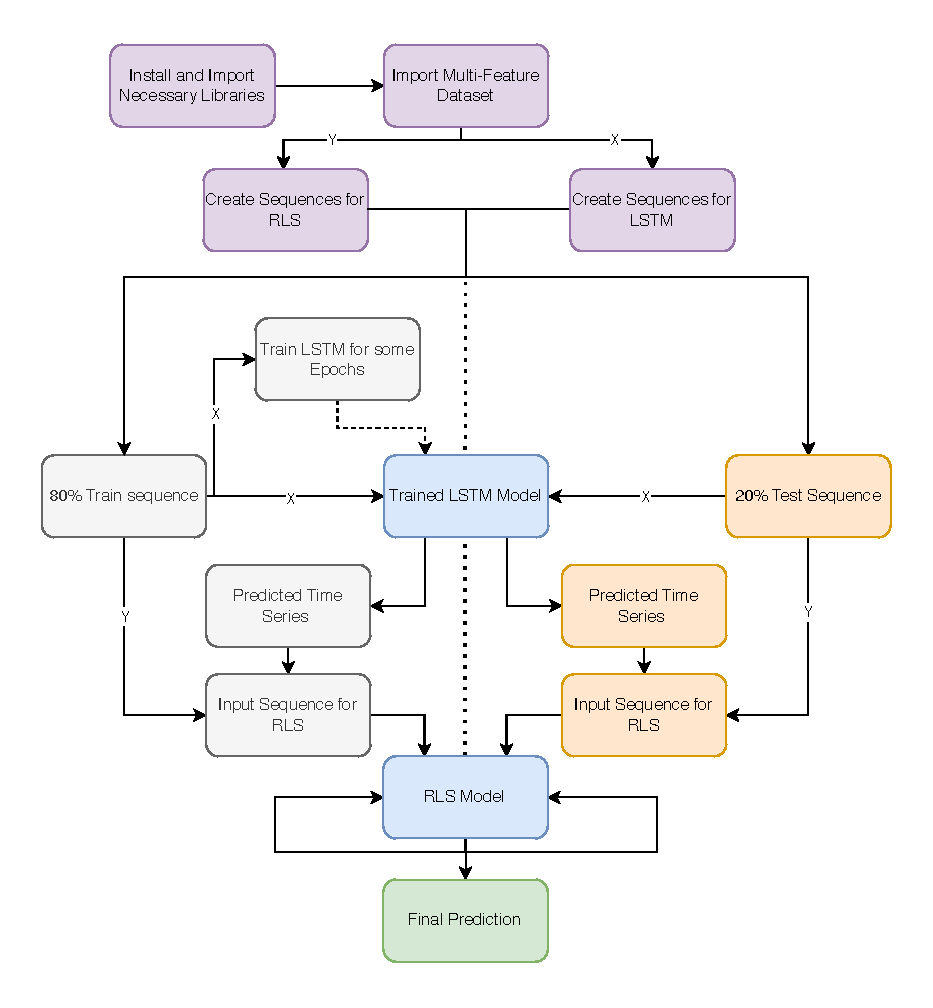
\includegraphics[width=0.8\textwidth]{Images/HybridLSTM_RLS_M.pdf}
    \caption{Flow diagram of Multi-Feature Hybrid LSTM-RLS implementation.}
    \label{fig:HybridLSTM_RLS_M}
\end{figure}

The LSTM model was trained following the standard sequence-based approach, where multi-feature input sequences were constructed and used for training.

\subsubsection{Key Modification: RLS Input Sequence Construction}

A significant deviation from the previous approach was the method used to construct input sequences for the \textbf{Recursive Least Squares (RLS) model}. As illustrated in \textbf{Figure~\ref{fig:RLS_Input_M}}, the input sequence creation for RLS followed a structured pipeline:

\begin{figure}[h!]
    \centering
    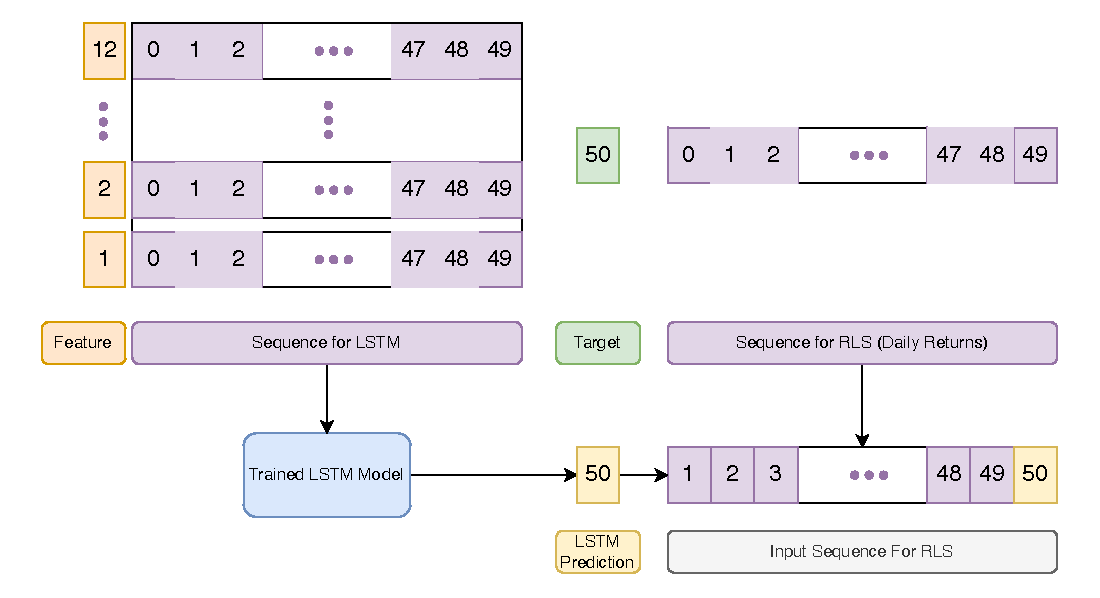
\includegraphics[width=0.8\textwidth]{Images/RLS_Input_M.pdf}
    \caption{RLS input sequence construction using LSTM outputs.}
    \label{fig:RLS_Input_M}
\end{figure}

\begin{itemize}
    \item Instead of deriving the RLS input sequences from the \textbf{LSTM input sequence}, the sequences were generated using \textbf{returns and close prices}.  
    \item The LSTM model was trained on sequences created from the \textbf{multi-feature input} (\textbf{X}). Once trained, the predicted values from LSTM were appended to the sequences constructed from \textbf{daily returns} (\textbf{Y}), ensuring that the RLS model receives inputs of the same nature as its output, thus allowing effective prediction in an online setting.
    \item Two separate training strategies were employed:  
    \begin{itemize}
        \item \textbf{Predicting Returns}: The model was trained to forecast stock returns, leveraging the structured relationship between past returns and future movements.  
        \item \textbf{Predicting Close Prices}: The model was also trained using close prices to evaluate its performance in direct price prediction.
    \end{itemize}
\end{itemize}

\subsubsection{Impact of this Approach}

\begin{itemize}
    \item \textbf{Alternative Feature Representation}: By constructing input sequences from returns and close prices, the model captured different aspects of market behavior.  
    \item \textbf{Comparative Performance Analysis}: Training for both returns and close prices allowed an in-depth evaluation of prediction effectiveness under different target variable choices.  
    \item \textbf{Flexible RLS Adaptation}: The RLS model benefited from this new input structure, enabling it to adjust dynamically to either return-based or price-based forecasts.  
\end{itemize}

This modification provided insights into how input sequence construction affects the overall model accuracy and adaptability, further refining the \textbf{Hybrid LSTM-RLS architecture}.

\section{Dual Network Solution (DNS) Architecture}
\subsection{Design and Integration}
The Dual Network Solution (DNS) architecture addresses the one-time-step lag observed in the previous models. Figure~\ref{fig:DNSArch} shows the DNS architecture, which involves two networks: one trained on trends and the other on actual data.

\begin{figure}[h!]
    \centering
    \includegraphics[width=0.8\textwidth]{Images/DNSArchitecture.pdf} % Adjust width as needed
    \caption{DNS Architecture}
    \label{fig:DNSArch}
\end{figure}

Steps include:
\begin{enumerate}
    \item \textbf{Trend extraction:} Network 1 is trained to predict trends using slope differences or moving averages.
    \item \textbf{Prediction refinement:} Network 2 uses the output of Network 1 to generate lag-free predictions.
\end{enumerate}

\section{Advanced Data Preprocessing for Enhanced Model Performance}
\subsection{Challenges in Scaling and Activation}
During the development of the stock price prediction models, challenges arose when scaling the data using traditional normalization techniques such as MinMaxScaler. This approach limits the range of predictions to the maximum value observed during training, potentially capping future predictions. To address this issue, an alternative preprocessing technique was introduced, which involves:
\begin{itemize}
    \item \textbf{Log Transformation:} Applying a logarithmic transformation to the close price values to reduce large variations and stabilize the data.
    \item \textbf{Standardization:} Standardizing the log-transformed values to ensure that the data is centered and scaled, allowing it to be processed effectively by the model.
\end{itemize}

After preprocessing, the resulting data ranged approximately between $-2$ and $2$. To handle this range, the \texttt{tanh} activation function was selected for its natural prediction range of $[-1, 1]$. However, to ensure flexibility in predictions beyond this range:
\begin{itemize}
    \item A multiplier of $2.5$ was applied after the \texttt{tanh} activation function. This adjustment extended the prediction range to $[-2.5, 2.5]$, providing additional room for extreme values without capping predictions.
\end{itemize}

Figure~\ref{fig:distribution_plot} shows the distribution plot of the raw close values, log-transformed close values, and scaled log-transformed values. This plot depicts how the preprocessing steps have allowed the data to fall in a range that the activation function can handle effectively.

\begin{figure}[h]
    \centering
    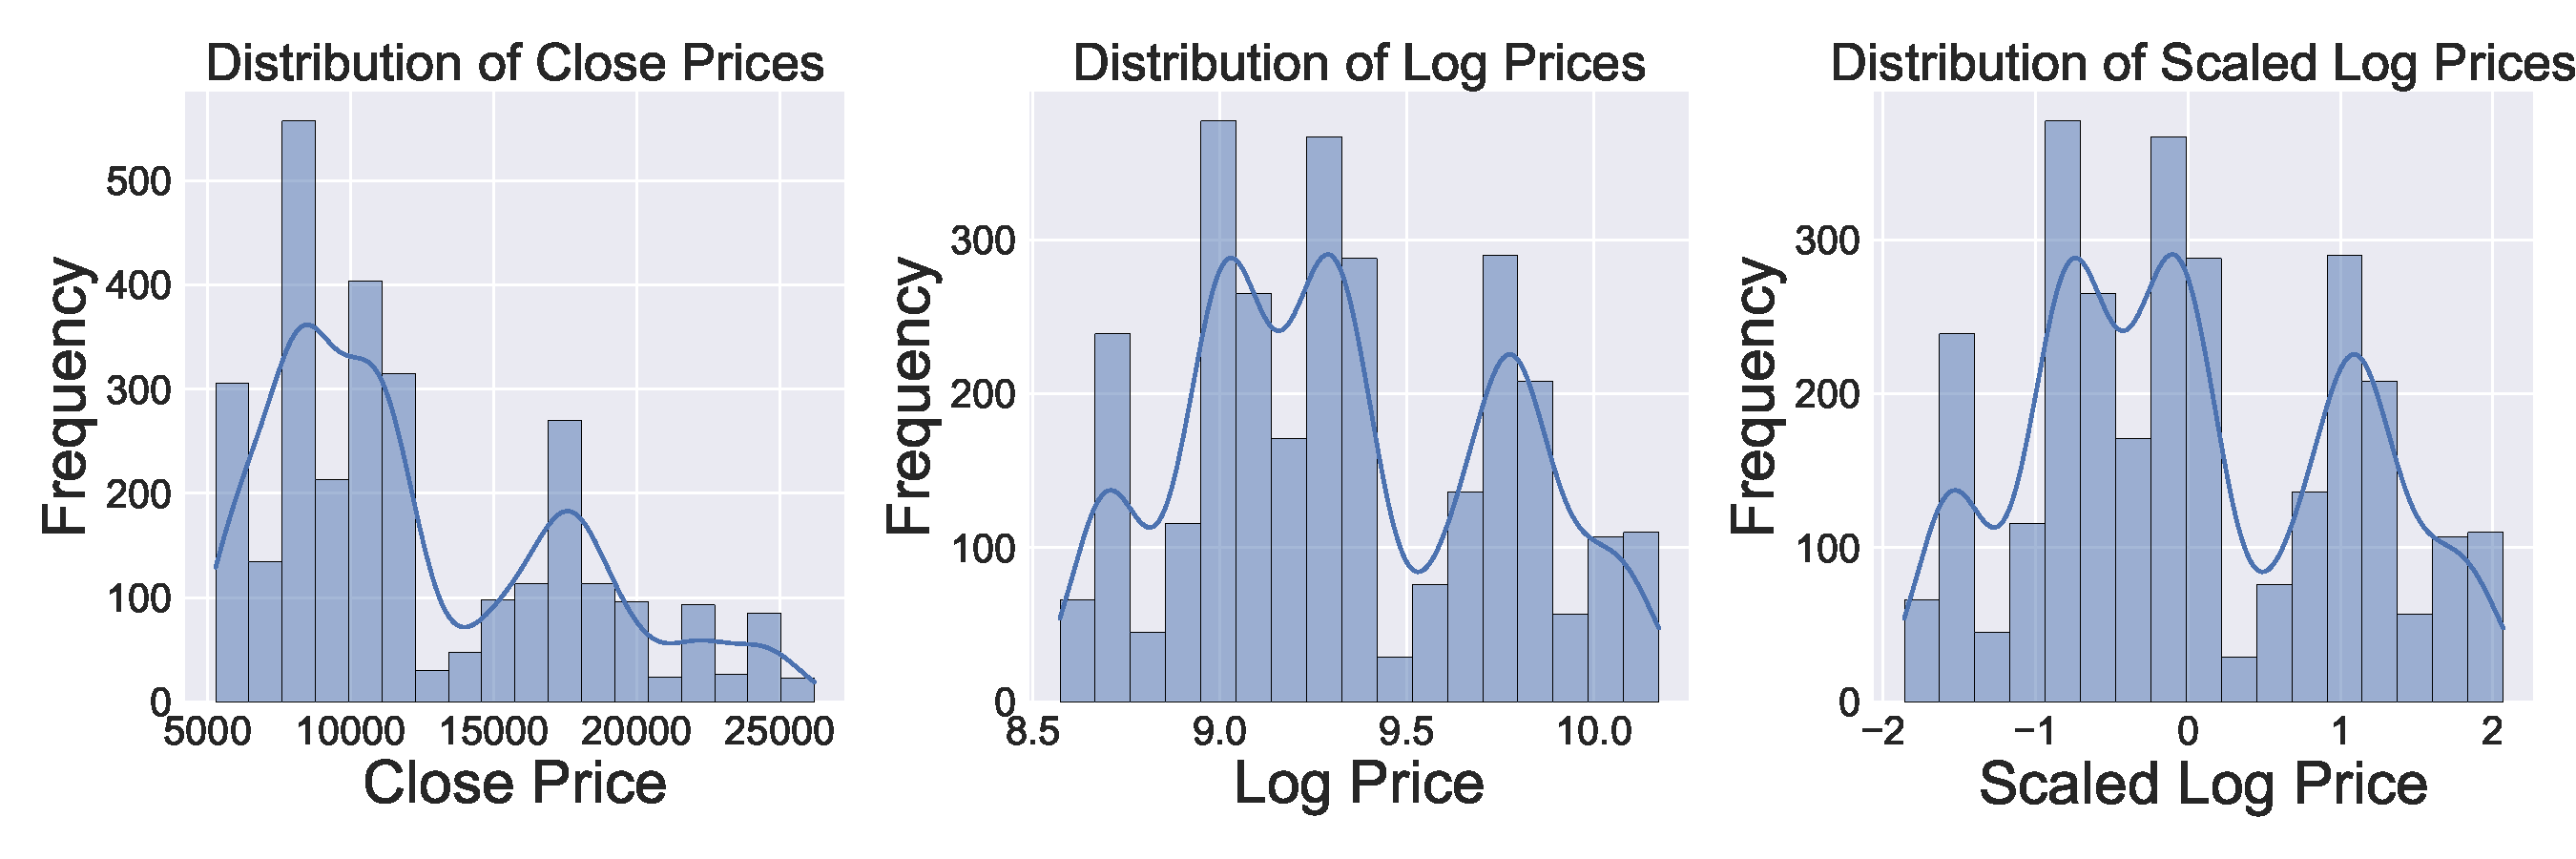
\includegraphics[width=\textwidth]{Images/distribution_plot.pdf}
    \caption{Distribution plot of raw close values, log-transformed close values, and scaled log-transformed close values.}
    \label{fig:distribution_plot}
\end{figure}

\subsection{Application in DNS Architecture}
This preprocessing technique, as explained in Section 3.5.1 was used in the concept of the Dual Network Solution Architecture. Using log transformation, standardization, and modified range of activation functions,
the DNS model represents both linear and nonlinear parts of
stock price movements.

This preprocess step was crucial in enhancing the prediction accuracy of the model.
racy of the DNS architecture, so that it could support a greater number of values
While the predictions of strength were retained, the changes had provided the basis for
groundwork for subsequent enhancements in model design and integration.


% \section{ARIMA-LSTM Residual Integration Framework}
% \subsection{Justification for ARIMA-LSTM Hybridization}
% This framework combines ARIMA's ability to model linear patterns with LSTM's strength in capturing non-linear relationships. The final prediction is obtained by integrating outputs from both models. Key components include:
% \begin{itemize}
%     \item \textbf{ARIMA model for linear trends:} ARIMA captures the linear component of stock prices.
%     \item \textbf{LSTM model for residuals:} LSTM models the non-linear residuals.
%     \item \textbf{Final integration:} Predictions from both models are combined for improved accuracy.
% \end{itemize}

\section{ARIMAX-LSTM Residual Integration Framework}
\subsection{ARIMAX-LSTM Hybridization}

The initial approach involved integrating the capability of ARIMA to model linear patterns and LSTM's strength in capturing non-linear relationships. However, due to suboptimal performance, the ARIMA model was replaced with ARIMAX for handling the linear component while LSTM continued to process residuals. The final prediction was obtained by integrating the outputs of these two models. The revised framework consists of:

\begin{itemize}
    \item \textbf{ARIMAX model for linear trends:} Unlike ARIMA, ARIMAX incorporates external features alongside past values to better capture the linear component of stock prices.
    \item \textbf{LSTM model for residuals:} LSTM models the remaining non-linear residuals after ARIMAX processing.
    \item \textbf{Final integration:} Predictions from both models are combined to enhance accuracy.
\end{itemize}

\subsection{Challenges and Model Refinement}

Initially, the ARIMA-LSTM hybrid model was tested; however, its performance was unsatisfactory. The residuals did not capture sufficient differences between the original close price values and ARIMA’s linear predictions, leading to subpar results. 

To address this issue:
\begin{itemize}
    \item The \textbf{ARIMA model was replaced with ARIMAX}, incorporating external variables to improve the modeling of linear relationships.
    \item The \textbf{LSTM model remained responsible for capturing non-linear residuals}.
    \item The integration of \textbf{ARIMAX and LSTM} was evaluated to determine if this modification led to improved performance.
\end{itemize}

This refined framework aimed to leverage ARIMAX's enhanced linear modeling alongside LSTM's capacity for non-linearity, ultimately improving the predictive capability of the model.

\subsection{Applying RLS to Residuals Framework Output}

In the \textbf{ARIMAX-LSTM-RLS model}, after predicting returns using the \textbf{ARIMA-LSTM Residual Integration Framework}, the next step involved incorporating \textbf{Recursive Least Squares (RLS)} to refine the final predictions.

\subsubsection{RLS Input Sequence Construction}

To enhance the prediction accuracy, input sequences for RLS were constructed as follows:
\begin{itemize}
    \item The predicted returns obtained from the \textbf{residuals architecture} were used to generate input sequences for RLS.
    \item RLS was then applied to these sequences, providing the \textbf{final predicted returns output}.
\end{itemize}

\subsubsection{Impact of RLS on the Residuals Architecture}

\begin{itemize}
    \item \textbf{Sequential Refinement}: By feeding the residuals architecture's output into RLS, the model aimed to further refine the predictions.
    \item \textbf{Performance Evaluation}: The final output from RLS was analyzed to determine whether this additional step improved the overall prediction accuracy.
\end{itemize}

This integration of RLS with the residuals architecture provided valuable insights into whether the additional layer of processing contributed to enhanced model performance.

% \section{Training Method for Multi-Feature LSTM Forecasting Framework}

% \subsection{One-Step Prediction and Incremental Training}

% In this framework, the primary focus is on one-step stock price prediction, as only the error between the next time step prediction and its actual value is significant for the application. Although the model forecasts multiple values in sequence, only the immediate next prediction is utilized in the algorithmic trading process. 

% Once the next day’s prediction is made, the following steps are performed to update the training and testing datasets:

% \begin{enumerate}
%     \item After the day ends, the actual value corresponding to the predicted value becomes available.
%     \item The first data point in the training set is discarded, and the current first data point from the testing dataset is appended to the training data.
%     \item Similarly, the first data point in the testing dataset is removed, and the latest actual value is added to it.
% \end{enumerate}

% This process ensures that the sizes of the training and testing datasets remain constant while incorporating the most recent data for improved accuracy. The model is then retrained daily after updating the datasets with the newly available data points.

% \subsection{Visualization of Incremental Training Process}

% The incremental training method is visualized in Figure~\ref{fig:incremental_training}, which provides a schematic representation of how the training and testing datasets are updated and retrained iteratively.

% \begin{figure}[h!]
%     \centering
%     \includegraphics[width=\textwidth]{incremental_training.pdf}
%     \caption{Visualization of the Incremental Training Process for Multi-Feature LSTM Forecasting Framework.}
%     \label{fig:incremental_training}
% \end{figure}

\section{Multi-Feature LSTM Forecasting Framework}
\subsection{Overview and Objectives}
The Multi-Feature LSTM Forecasting Framework aims to enhance stock price prediction accuracy by incorporating a diverse set of features derived from technical indicators and price patterns. These features include daily returns, Relative Strength Index (RSI), On-Balance Volume (OBV), and various ratios capturing short-term and long-term price movements. 

The key objectives of this framework are:
\begin{itemize}
    \item Many key features for an integrated understanding of
Market Behavior.
    \item Developing a methodology of training that is robust and adaptive for daily usage.
    \item It uses the strength of LSTM in capturing temporal dependency.
cies within financial data.
\end{itemize}

The framework is designed based on the model's adaptability with respect to newer ideas. Market trend with scalability and computational effectiveness of a solution.
Incorporation of feature selection and refinement adds further sophistication to the predictivity ability of the model.

\subsection{Training Methodology}
This is specific for the Multi-Feature LSTM Forecasting Framework. Designed for high-level real-time stock market information processing and daily changes. The methodology involved the following:
\subsubsection{One-Step Prediction and Incremental Training}
That makes the prediction of the stock price at the next step a function of only
Minimize the error between the predicted and actual values for the immediate next day. Even though it is predicting several future time steps, only the first
The predicted value is used in the context of algorithmic trading for decision making.
Immediately after obtaining tomorrow's true value, the training and testing datasets
are updated:
\begin{enumerate}
    \item Function that omits the first value in the training dataset and the last value from the test dataset is appended to keep the no of training sample sizes.
    \item The first value in the test data set is removed, and the newly
real value is returned by the final entry of available.
\end{enumerate}

This means the model is updated on the most recently available data points.
It enables it to adjust to changes in the market. The model is trained daily
With such an updated dataset, predictions of the following day can be made

\subsubsection{Visualization of Incremental Training Process}
The incremental training process is visualized in Figure~\ref{fig:incremental_training}. This figure illustrates the dynamic updates to the training and testing datasets as new data becomes available. The real-time adaptability of the model is a key feature that supports its application in live trading environments.

\begin{figure}[h!]
    \centering
    \includegraphics[width=\textwidth]{Images/incremental_training.pdf}
    \caption{Visualization of the Incremental Training Process for Multi-Feature LSTM Forecasting Framework.}
    \label{fig:incremental_training}
\end{figure}

\subsection{Feature Engineering Techniques}
This framework incorporates multiple features, such as returns, RSI, and OBV, to enhance predictive accuracy. All features were normalized for consistency. 

The distribution of all features in the dataset is shown in Figure~\ref{fig:feature_distributions}. This plot highlights the range and variability of each feature, demonstrating the effectiveness of normalization.

\begin{figure}[h!]
    \centering
    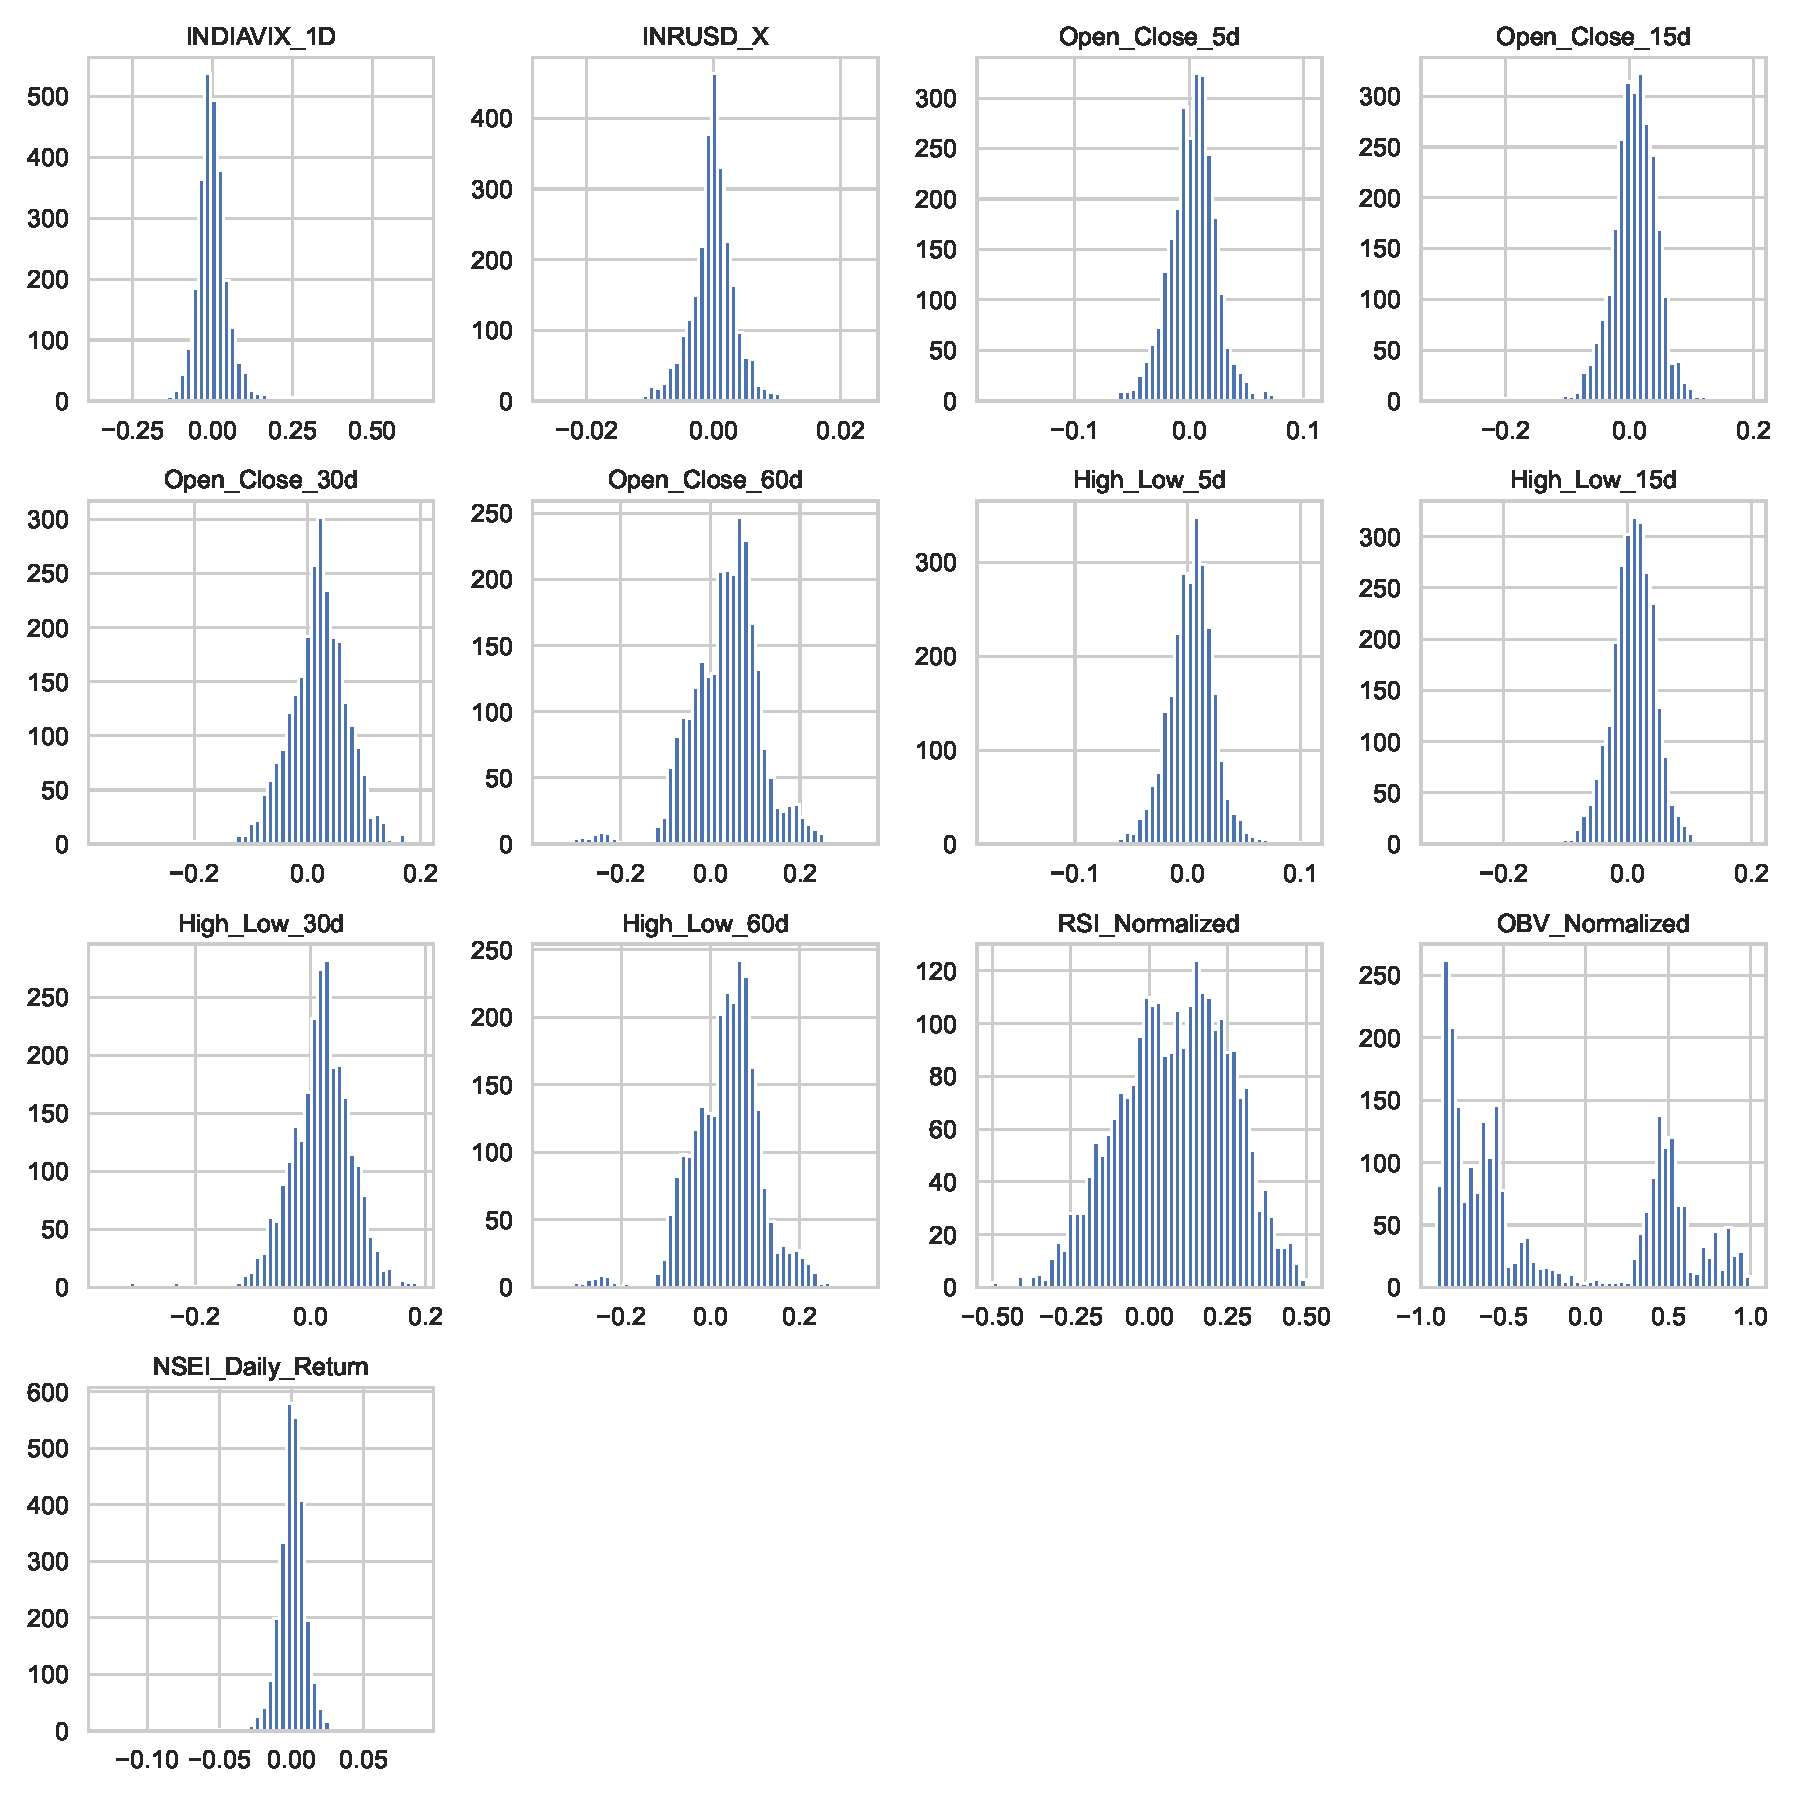
\includegraphics[width=\textwidth]{Images/feature_distributions.pdf}
    \caption{Distribution plots of all features used in the forecasting framework.}
    \label{fig:feature_distributions}
\end{figure}

Additionally, the correlation matrix for all features is displayed in Figure~\ref{fig:correlation_plot}. This plot provides insights into feature interdependencies and the strength of their relationships with the target variable.

\begin{figure}[h!]
    \centering
    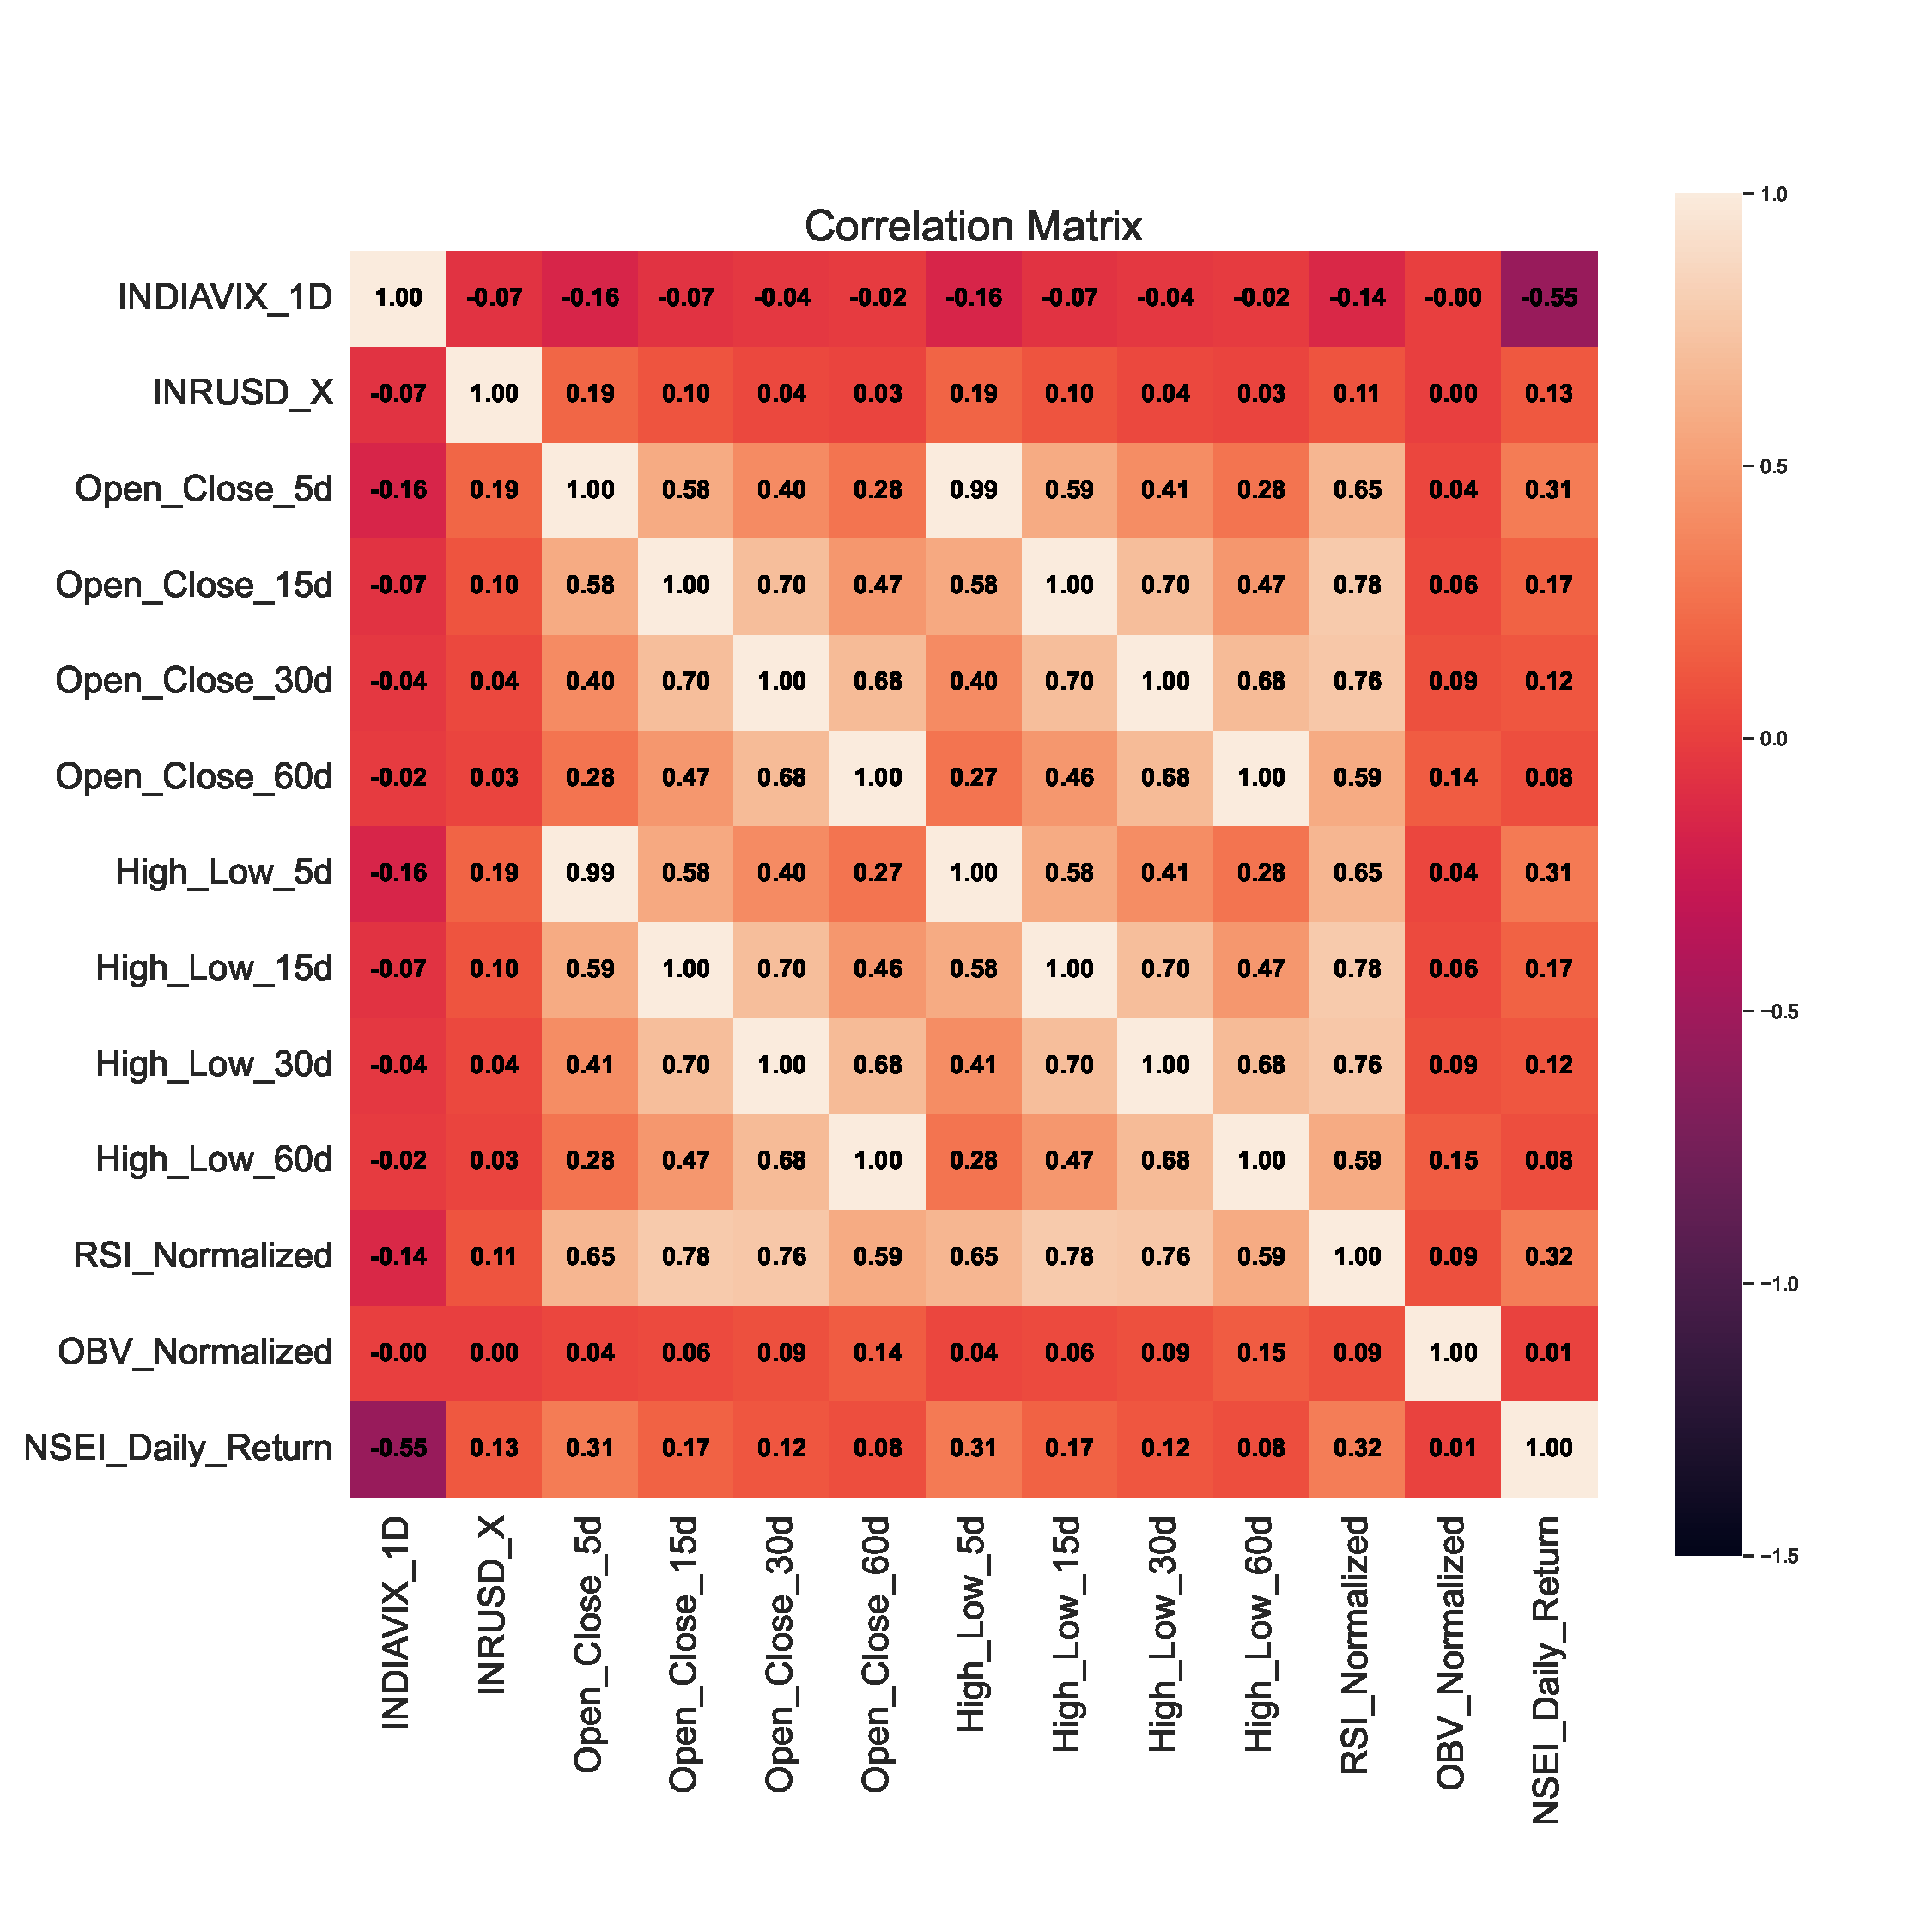
\includegraphics[width=\textwidth]{Images/correlation_plot.pdf}
    \caption{Correlation matrix of all features in the dataset.}
    \label{fig:correlation_plot}
\end{figure}

Finally, Figure~\ref{fig:seasonal_decomposition} presents the seasonal decomposition plot of NSEI close values, illustrating the observed trend, seasonality, and residual components. This visualization assists in understanding the underlying temporal patterns of the target variable.

\begin{figure}[h!]
    \centering
    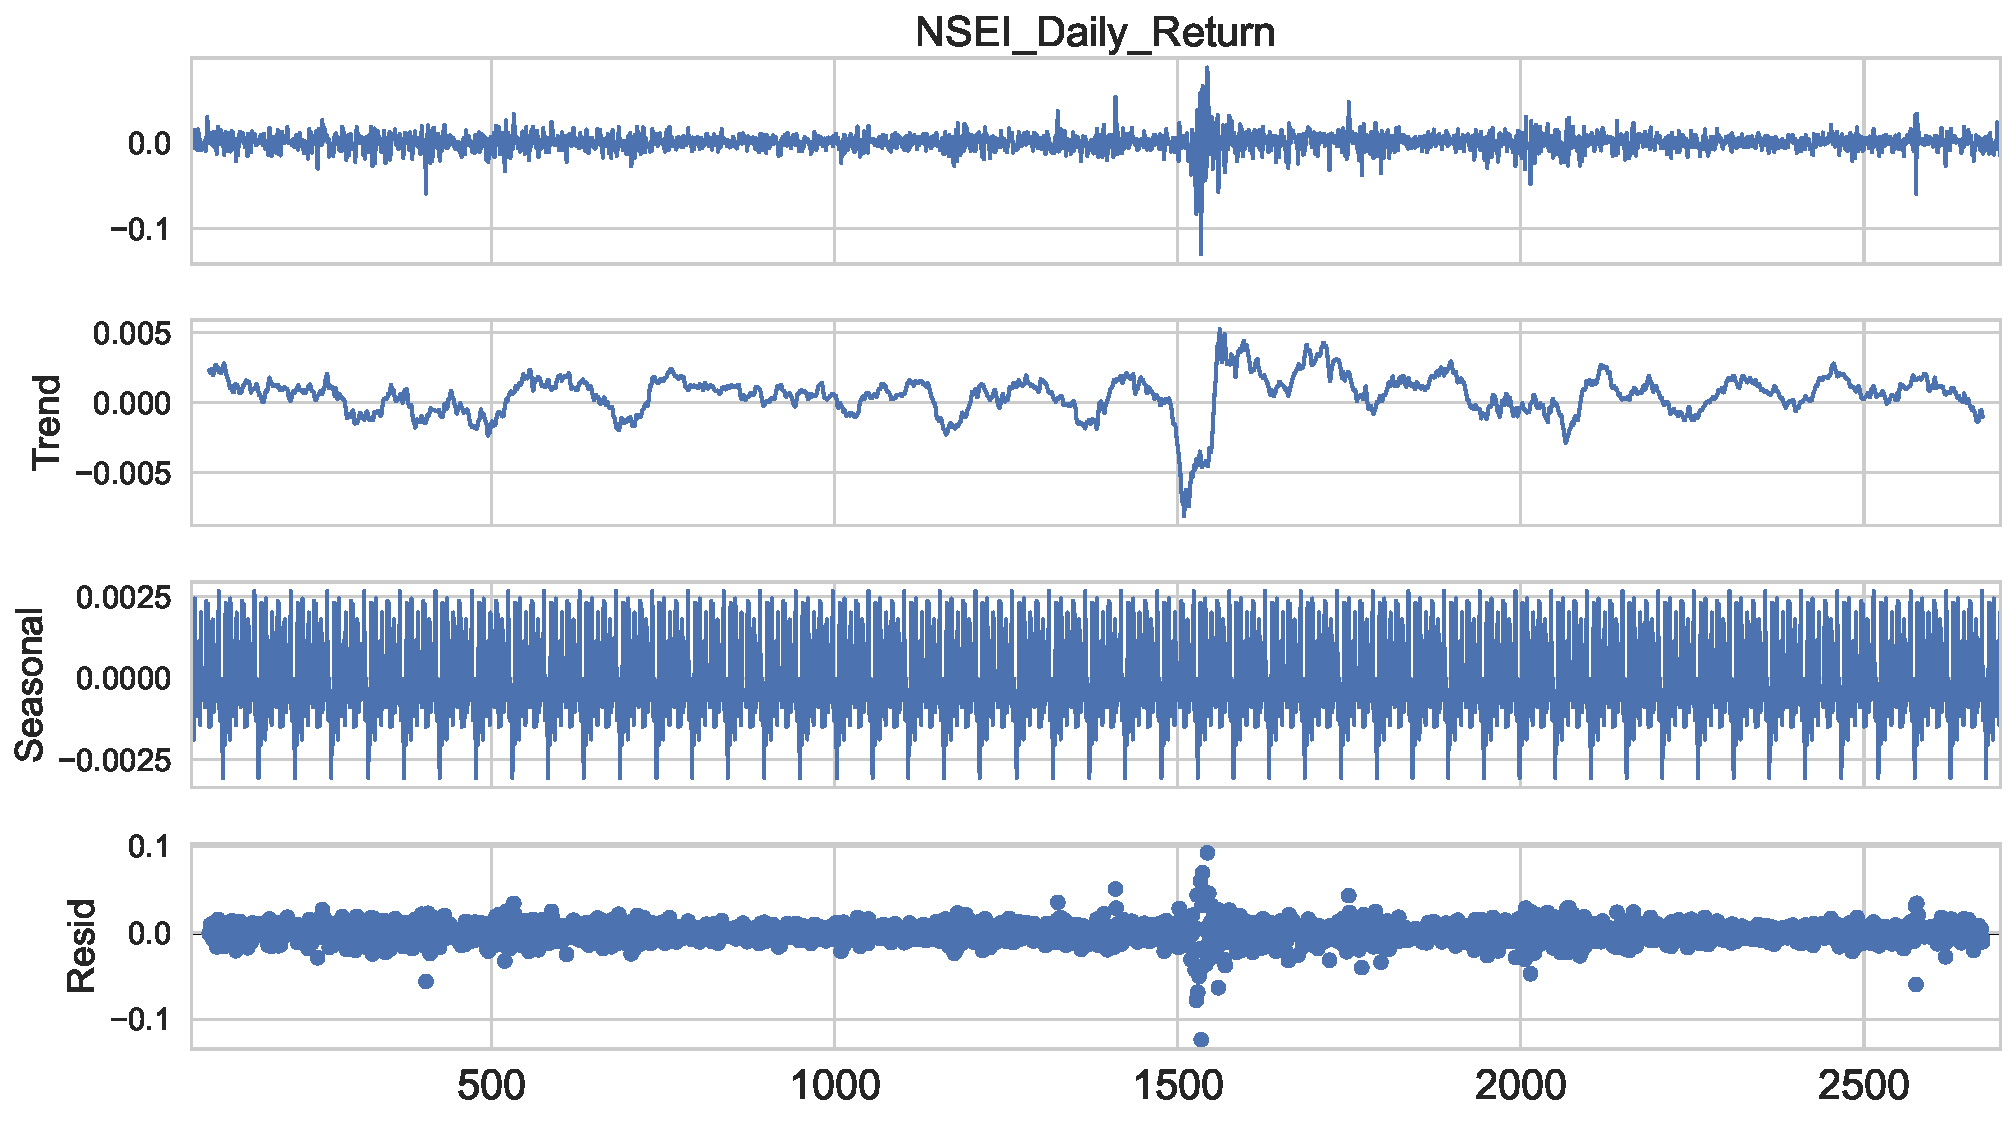
\includegraphics[width=\textwidth]{Images/seasonal_decomposition.pdf}
    \caption{Seasonal decomposition of NSEI close values.}
    \label{fig:seasonal_decomposition}
\end{figure}

\subsection{Feature Selection Using SelectKBest}
Feature selection was performed using the SelectKBest method with \texttt{f\_regression}. The feature importance scores are presented in Table~\ref{tab:feature_importance}.

\begin{table}[h!]
\centering
\caption{Feature Importance Scores using SelectKBest}
\begin{tabular}{|l|c|}
\hline
\textbf{Feature} & \textbf{Score} \\ \hline
INDIAVIX\_1D     & 1125.250181    \\ \hline
RSI\_Normalized  & 292.775295     \\ \hline
Open\_Close\_5d  & 276.984547     \\ \hline
High\_Low\_5d    & 268.947328     \\ \hline
High\_Low\_15d   & 79.876745      \\ \hline
Open\_Close\_15d & 79.634278      \\ \hline
INRUSD\_X        & 42.357608      \\ \hline
Open\_Close\_30d & 35.719346      \\ \hline
High\_Low\_30d   & 35.259659      \\ \hline
Open\_Close\_60d & 16.824506      \\ \hline
High\_Low\_60d   & 16.235917      \\ \hline
OBV\_Normalized  & 0.570088       \\ \hline
\end{tabular}

\label{tab:feature_importance}
\end{table}

\subsection{Feature Refinement}
Low-importance features such as OBV\_Normalized and 30-day/60-day returns were dropped. The refined feature set ensured better model performance with reduced complexity.

\section{GARCH for Stock Price Prediction}

\subsection{Introduction to GARCH}

The Generalized Autoregressive Conditional Heteroskedasticity (GARCH) model is widely used in financial time series modeling due to its ability to capture volatility clustering. In stock markets, volatility tends to persist over time, meaning that periods of high volatility are often followed by more volatile periods, and similarly for low volatility. Since the target variable in this study is \textbf{daily returns}, which inherently exhibits volatility characteristics, GARCH is a suitable choice for modeling this behavior.

GARCH is particularly relevant to this study because it models conditional variance, providing insights into future uncertainty levels. By leveraging GARCH, we aim to enhance stock return prediction by explicitly modeling the variance dynamics, which traditional models might overlook.

\subsection{Model Implementation}

To implement GARCH, the following approach was used:

\begin{itemize}
    \item \textbf{Mean Prediction using ARIMAX:} Before applying GARCH, the mean component of stock returns was modeled using the ARIMAX model. ARIMAX extends ARIMA by incorporating external regressors, making it suitable for capturing linear dependencies in stock returns.
    \item \textbf{Residuals Extraction:} After obtaining the ARIMAX predictions, the residuals (unexplained variations) were extracted. These residuals capture the unpredictable fluctuations in returns.
    \item \textbf{GARCH Modeling on Residuals:} The extracted residuals were then used to train a GARCH model, which estimated the conditional variance of the returns. The GARCH model accounted for volatility clustering, ensuring that periods of high variance were correctly modeled.
\end{itemize}

\subsection{Integration with Existing Architectures}

The GARCH model was not used in isolation but was integrated into the broader framework of stock price prediction. Specifically:

\begin{itemize}
    \item The \textbf{ARIMAX model} was used for predicting the mean returns.
    \item The \textbf{GARCH model} was applied to the residuals from ARIMAX to model volatility.
    \item The final output was a combination of the ARIMAX-predicted mean and the variance estimation from the GARCH model, providing a more comprehensive prediction of stock returns.
\end{itemize}

By integrating GARCH with ARIMAX, the model was able to separately handle both the trend and volatility components of stock returns, improving the overall robustness of the forecasting framework.



% \chapter{Frameworks and Models for Stock Price Prediction}

% \section{Overview of Proposed Architectures}
% This chapter provides a detailed explanation of various architectures designed and developed for stock price prediction. Starting from the Hybrid LSTM-RLS Architecture created during the summer internship, subsequent modifications and alternative models are described, highlighting their strengths, limitations, and outcomes.

% \section{Hybrid LSTM-RLS Architecture}

% \subsection{Workflow and Design}

% The Hybrid LSTM-RLS architecture was developed during my summer internship. It combines the strengths of Long Short-Term Memory (LSTM) networks for sequential data modeling with Recursive Least Squares (RLS) for refining predictions.

% \begin{figure}[h!]
%     \centering
%     \includegraphics[width=0.8\textwidth]{SummerInternArchitecture.pdf} % Adjust width as needed
%     \caption{Hybrid LSTM-RLS Architecture}
% \label{fig:summerarch}
% \end{figure}

% Figure \ref{fig:summerarch} illustrates the workflow of this architecture. Key steps are as follows:
% \begin{enumerate}
%     \item \textbf{Install and load necessary libraries:} 
%     \begin{itemize}
%         \item Libraries such as tensorflow, numpy, yfinance and scikit- learn are installed and imported.
%     \end{itemize}
    
%     \item \textbf{Load stock data using yfinance API:} 
%     \begin{itemize}
%         \item Data representing price of the stocks in any given time is extracted from yfinance API for the desired time.
%     \end{itemize}
    
%     \item \textbf{Data preprocessing:} 
%     \begin{itemize}
%         \item Preprocessing of data is also performed, which consists of normalization, missing values dealt and the splitting of data in training and testing.
%     \end{itemize}
    
%     \item \textbf{Create sequences:}
%     \begin{itemize}
%         \item Price sequences of stocks are generated for making the data ready for LSTM
% model. Every one of these sequences includes information about the past price level for training purposes.
%     \end{itemize}
    
%     \item \textbf{Train the LSTM model:}
%     \begin{itemize}
%         \item Using these sequences, LSTM model is prepared and tested for predicting the next value of the stock.
%     \end{itemize}
    
%     \item \textbf{LSTM predictions passed to RLS model:}
%     \begin{itemize}
%         \item The scalar predictions from the LSTM model are taken as an input by the RLS algorithm.
%     \end{itemize}
    
%     \item \textbf{RLS model provides final prediction:}
%     \begin{itemize}
%         \item The RLS model processes the LSTM prediction and from it produces the final stock price prediction.
%     \end{itemize}
    
% \end{enumerate}

% \section{Enhanced Hybrid LSTM-RLS Architecture}

% To address issues such as dimension mismatches and long training times in the original architecture, several enhancements were implemented in Semester 3. These refinements simplified the process and improved predictive accuracy.

% Figure \ref{fig:Refinedarch} illustrates the improved workflow:

% After I started Semester 3, I improved the architecture developed in this early figure \ref{fig:Refinedarch}. Such improvements were executed to make the architecture more predictable and to solve problems such as dimension mismatch and long training times. It made the model much simpler and highly efficient to use for stock price forecasting.

% \subsection{Architecture Workflow}

% \begin{figure}[htbp]
%     \centering
%     \includegraphics[width=0.8\textwidth]{RefinedArchitecture.pdf} % Adjust width as needed
%     \caption{Enhanced Hybrid LSTM-RLS Architecture}
% \label{fig:Refinedarch}
% \end{figure}

% Architecture process involves the following steps:

% \begin{enumerate}
%     \item \textbf{Install and import necessary libraries:}
%     \begin{itemize}
%         \item All libraries are imported as like yfinance, tensorflow, scikit-learn and so on.
%     \end{itemize}
    
%     \item \textbf{Import Nifty 50 daily close price data:}
%     \begin{itemize}
%         \item For the last 12 years, it fetches the closing prices of Nifty 50 from the yfinance API daily.
%     \end{itemize}
    
%     \item \textbf{Normalize the data:}
%     \begin{itemize}
%         \item Normalized the data and scaled it between 0 to 1 and fed it into the LSTM model. This was done using MinMaxScaler.
%     \end{itemize}
    
%     \item \textbf{Create sequences for LSTM:}
%     \begin{itemize}
%         \item Sequences of past stock prices are created to prepare the data for LSTM training.
%     \end{itemize}
    
%     \item \textbf{Divide the data into 80\% training and 20\% testing:}
%     \begin{itemize}
%         \item The sequences are divided into 80\% for training and 20\% for testing.
%     \end{itemize}
    
%     \item \textbf{Train the LSTM model:}
%     \begin{itemize}
%         \item The LSTM model is trained on the 80\% training data over several epochs to predict the stock prices.
%     \end{itemize}
    
%     \item \textbf{Use LSTM to forecast:}
%     \begin{itemize}
%         \item The trained LSTM model provides predictions for both the train and test sets.
%     \end{itemize}
    
%     \item \textbf{Sequences used in RLS model input:}
%     \begin{itemize}
%         \item The LSTM model predictions are used to create input sequences for the Recursive Least Squares (RLS) model.
%     \end{itemize}
    
%     \item \textbf{Forecast final stock prices using the RLS model:}
%     \begin{itemize}
%         \item The RLS model uses the LSTM predictions as input and outputs the final stock price predictions.
%     \end{itemize}
    
% \end{enumerate}

% \subsection{Developing Input Sequences for RLS}

% \begin{figure}[htbp]
%     \centering
%     \includegraphics[width=0.8\textwidth]{RLSInputCreation.pdf} % Adjust width as needed
%     \caption{Input Sequence Formation}
% \label{fig:inputseq}
% \end{figure}

% The following steps are followed to generate the input sequences for the RLS model based on LSTM predictions:

% \begin{enumerate}
%     \item \textbf{Original Sequence for LSTM:} 
%     \begin{itemize}
%         \item The original sequence of stock prices is used as the input to the LSTM model. 
%         \item For example, a sequence from index 0 to 49 is selected.
%     \end{itemize}

%     \item \textbf{Training the LSTM Model:}
%     \begin{itemize}
%         \item The LSTM model is trained on the input sequence.
%         \item After training, the LSTM model generates a prediction, i.e., the 50th value based on the past 49 values.
%     \end{itemize}

%     \item \textbf{Shifting the Sequence for RLS Input:}
%     \begin{itemize}
%         \item The sequence used for LSTM training is shifted by one step to create the input for the RLS model.
%         \item For instance, the sequence now starts from index 1 and runs up to index 50.
%         \item The prediction generated by the trained LSTM model for the 50th point is appended to this new sequence.
%     \end{itemize}

%     \item \textbf{Final Input for RLS Model:}
%     \begin{itemize}
%         \item The shifted sequence (from 1 to 50) is provided as input to the RLS model.
%         \item The RLS model uses this input to generate the final stock price prediction.
%     \end{itemize}
% \end{enumerate}

% This process enables the integration of the LSTM predictions with the RLS model by using a sequential sliding window approach.

% \section{Dual Network Solution Architecture}
% The RMSE and R\(^2\) score of the Enhanced Hybrid LSTM-RLS architecture show good performance, but there exists a constant lag of 1 time step in the predictions. This results in a relatively higher RMSE error of 0.76\%. To address this lag, I adopted the Dual Network Solution (DNS) architecture proposed by \textcite{samanta_dual_2020}, which is designed to reduce such time-step lags in forecasting.

% Figure \ref{fig:DNSArch} illustrates the architecture of the Dual Network Solution (DNS) Architecture, which operates as follows:

% \begin{enumerate}
%     \item \textbf{Training Network 1}: 
%     Network 1 is trained on trends extracted from actual data using the Slope Difference Method or Moving Averages.
    
%     \item \textbf{Training Network 2}: 
%     Network 2 is trained directly on the actual data.
    
%     \item \textbf{Lag-Free Prediction}: 
%     After training, the models are used for lag-free predictions.
    
%     \item \textbf{Input to Network 1}: 
%     The actual data is passed as input to Network 1, which predicts the trend based on this input.
    
%     \item \textbf{Input to Network 2}: 
%     The predicted trend from Network 1 is then provided as input to Network 2 to obtain the final prediction.
% \end{enumerate}

% \begin{figure}[htbp]
%     \centering
%     \includegraphics[width=0.8\textwidth]{23MAI004_Sem3_MidSem_Report/DNSArchitecture.pdf} % Adjust width as needed
%     \caption{DNS Architecture}
% \label{fig:DNSArch}
% \end{figure}

% \section{ARIMA-LSTM Residual Integration Framework}

% In this section, I have employed a hybrid model aimed at addressing the lag observed in the results of the Dual Network Solution (DNS) architecture discussed previously. The model architecture used here is inspired by the framework proposed by Shah et al. In their approach, the authors decompose the final stock price prediction into three components: \textbf{linear}, \textbf{non-linear}, and \textbf{error}.

% \begin{itemize}
%     \item \textbf{Linear Component}: The ARIMA model is employed to make an initial prediction by capturing the linear component in the data. The residuals are then computed as the difference between the actual values and the ARIMA predictions.  
%     \item \textbf{Non-linear Component}: The calculated residuals are used as input to an LSTM model, which is trained to capture the non-linear component of the data.  
%     \item \textbf{Final Prediction}: The predictions from the ARIMA model and the LSTM model are combined to obtain the final stock price predictions.
% \end{itemize}

% To build upon this framework, I have made modifications by employing the LSTM model to predict both the linear and non-linear components of the data. This adjustment aims to enhance the model’s flexibility and predictive accuracy. The complete flow of the proposed architecture, including its modifications, is illustrated in \textbf{Figure 1}.

% \section{Multi-Feature LSTM Forecasting Framework}

% As the \textbf{ARIMA-LSTM Residual Integration Framework} was unable to effectively remove the lag in predictions and its performance degraded compared to other proposed models, I decided to adopt a \textbf{Multi-Feature LSTM Forecasting Framework}. This approach utilizes multiple features as input to train the LSTM architecture, aiming to improve the predictive accuracy and eliminate lag.

% \subsection{Feature Engineering}

% The dataset includes the following features:
% \begin{itemize}
%     \item \textbf{5-day, 15-day, 30-day, and 60-day returns} calculated using the average of high and low values of NSEI.
%     \item \textbf{5-day, 15-day, 30-day, and 60-day returns} calculated using the average of open and close values of NSEI.
%     \item \textbf{RSI (Relative Strength Index)} values calculated on daily close values, normalized to a range of \([-0.5, 0.5]\).
%     \item \textbf{OBV (On-Balance Volume)} values calculated using close values and volume of NSEI, normalized to a range of \([-1, 1]\).
%     \item \textbf{1-day returns} calculated on daily close values of INR-USD currency exchange data.
%     \item \textbf{1-day returns} calculated on daily close values of the \(^\text{INDIAVIX}\) index.
% \end{itemize}

% All return values were kept in their original scale, while RSI and OBV were normalized for consistency.

% The entire dataset is visualized using histograms, correlation plots, and pair plots, which are shown below.


% \subsection{Feature Selection Using SelectKBest}

% To refine the dataset, I applied the \textbf{SelectKBest} feature selection method with \texttt{f\_regression} as the scoring function. The input features were evaluated against the daily returns calculated on daily close values of NSEI as the output. The importance scores of the features are presented in Table~\ref{tab:feature_importance}.

% \begin{table}[H]
% \centering
% \begin{tabular}{|l|c|}
% \hline
% \textbf{Feature} & \textbf{Score} \\ \hline
% INDIAVIX\_1D     & 1125.250181    \\ \hline
% RSI\_Normalized  & 292.775295     \\ \hline
% Open\_Close\_5d  & 276.984547     \\ \hline
% High\_Low\_5d    & 268.947328     \\ \hline
% High\_Low\_15d   & 79.876745      \\ \hline
% Open\_Close\_15d & 79.634278      \\ \hline
% INRUSD\_X        & 42.357608      \\ \hline
% Open\_Close\_30d & 35.719346      \\ \hline
% High\_Low\_30d   & 35.259659      \\ \hline
% Open\_Close\_60d & 16.824506      \\ \hline
% High\_Low\_60d   & 16.235917      \\ \hline
% OBV\_Normalized  & 0.570088       \\ \hline
% % Unnamed: 0       & 0.075218       \\ \hline
% \end{tabular}
% \caption{Feature Importance Scores using SelectKBest}
% \label{tab:feature_importance}
% \end{table}

% \subsection{Feature Refinement}

% Based on the feature importance scores, the following features were dropped due to their low relevance:
% \begin{itemize}
%     \item \textbf{OBV\_Normalized}: Score of 0.570088.
%     \item \textbf{30-day and 60-day returns} calculated for both \textbf{open-close} and \textbf{high-low} averages.
% \end{itemize}

% The refined feature set focuses on the most important predictors, ensuring improved model performance while reducing complexity.
% \chapter{Results and Publications}

% \section{Evaluation Matrix}
% \subsubsection*{Root Mean Squared Error (RMSE)}
% On this basis, the Root Mean Squared Error (RMSE) is an evaluation criterion with reference to the accuracy of the model’s forecast. It is actually the square root of the arithmetic mean of the squared difference between them and the predicted values. RMSE offers further information to do with unequal trifling with the scale of data especially for regression models, in circumstance of absolute mistakes. It is defined as follows:

% \begin{equation}
% \text{RMSE} = \sqrt{\frac{1}{n} \sum_{i=1}^{n} (y_i - \hat{y}_i)^2}
% \end{equation}

% where:
% \begin{itemize}
%     \item \( n \) is the number of observations,
%     \item \( y_i \) is the actual value of the \(i^{th}\)observation,
%     \item \( \hat{y}_i \) is the predicted value of the \(i^{th}\) observation.
% \end{itemize}

% \subsubsection*{R-squared (R²)}
% The coefficient of multiple determination R² is an R statistic the measures percentage or proportion of variance in the dependent/forecasted variable, explained by the changes in one or organisms independent/predictor variable. It helps us to know how well the regression model has been fitted into the data. The Squared Multiple Correlation values has a range of 0 – 1 where the value of 1 mean all variations have been explained by the model while the value 0 means no variation in the data has been explained by the model. Another measure of the reliability of the model can also be estimate from the statistic R² whereby a higher value is preferred. It is
% defined as follows:

% \begin{equation}
% R^2 = 1 - \frac{\sum_{i=1}^{n} (y_i - \hat{y}_i)^2}{\sum_{i=1}^{n} (y_i - \bar{y})^2}
% \end{equation}

% where:
% \begin{itemize}
%     \item \( n \) stands the number of observations,
%     \item \( y_i \) stands for the true value the \(i^{th}\) observation,
%     \item \( \hat{y}_i \) stands the predicted value of the \(i^{th}\) observation,
%     \item \( \bar{y} \) stands the mean of the actual values.
% \end{itemize}

% \section{Enhanced Hybrid LSTM-RLS Architecture Results}


% Figure \ref{fig:refinedApproachRes1} and \ref{fig:refinedApproachRes2} brings out the performance of the model in terms of identifying the patterns during training, which is reflected in the high R² score.

% % Modify figure sizes according to your needs
% \begin{figure}[h!]
%     \centering
%     \includegraphics[width=\textwidth]{23MAI004_Sem3_MidSem_Report/ActvsPred.pdf}
%     \caption{ Original vs. Predicted Stock Prices }
%     \label{fig:refinedApproachRes1}
% \end{figure}

% \begin{figure}[h!]
%     \centering
%     \includegraphics[width=\textwidth]{23MAI004_Sem3_MidSem_Report/returns_comparision.pdf}
%     \caption{ Returns: Original vs. Predicted Prices }
%     \label{fig:refinedApproachRes2}
% \end{figure}

% Table \ref{tab:lstm_rls_performance} and Table \ref{tab:bi_lstm_rls_performance} show the results of the Hybrid LSTM-RLS model (both LSTM and Bi-LSTM) when the architecture is tested on the test data. The results include RMSE for daily close prices and RMSE when both actual and predicted values are converted into returns, and then the RMSE is calculated between them.

% \begin{table}[h!]
% \centering
% \begin{tabular}{|l|c|c|c|}
% \hline
% \textbf{LSTM-RLS}  & \textbf{Daily Returns} & \textbf{Weekly Returns} & \textbf{Daily Close} \\ \hline
% \textbf{RMSE}      & 0.76\%                 & 1.44\%                 & 161.8935             \\ \hline
% \textbf{R2}        & -0.0636                & -0.038                 & 0.9956               \\ \hline
% \end{tabular}
% \caption{LSTM-RLS Performance Metrics}
% \label{tab:lstm_rls_performance}
% \end{table}

% \begin{table}[h!]
% \centering
% \begin{tabular}{|l|c|c|c|}
% \hline
% \textbf{\textit{Bi-LSTM - RLS}} & \textbf{Daily Returns} & \textbf{Weekly Returns} & \textbf{Daily Close} \\ \hline
% \textbf{RMSE}                   & 0.77\%                 & 2.22\%                 & 161.7337             \\ \hline
% \textbf{R2}                     & -0.0879                & -1.4785                & 0.9956               \\ \hline
% \end{tabular}
% \caption{Bi-LSTM - RLS Performance Metrics}
% \label{tab:bi_lstm_rls_performance}
% \end{table}

% \section{Results with Shift}

% Figures~\ref{fig:revisedApproachshift1} and \ref{fig:revisedApproachshift2} represent the actual daily close versus shifted predicted daily close, and returns calculated on actual daily close versus returns calculated on shifted predicted daily close, respectively.

% % Modify figure sizes according to your needs
% \begin{figure}[h!]
%     \centering
%     \includegraphics[width=\textwidth]{23MAI004_Sem3_MidSem_Report/ActvsPredshift.pdf}
%     \caption{ Stock Prices: Shifted Predictions (-1)}
%     \label{fig:revisedApproachshift1}
% \end{figure}

% \begin{figure}[h!]
%     \centering
%     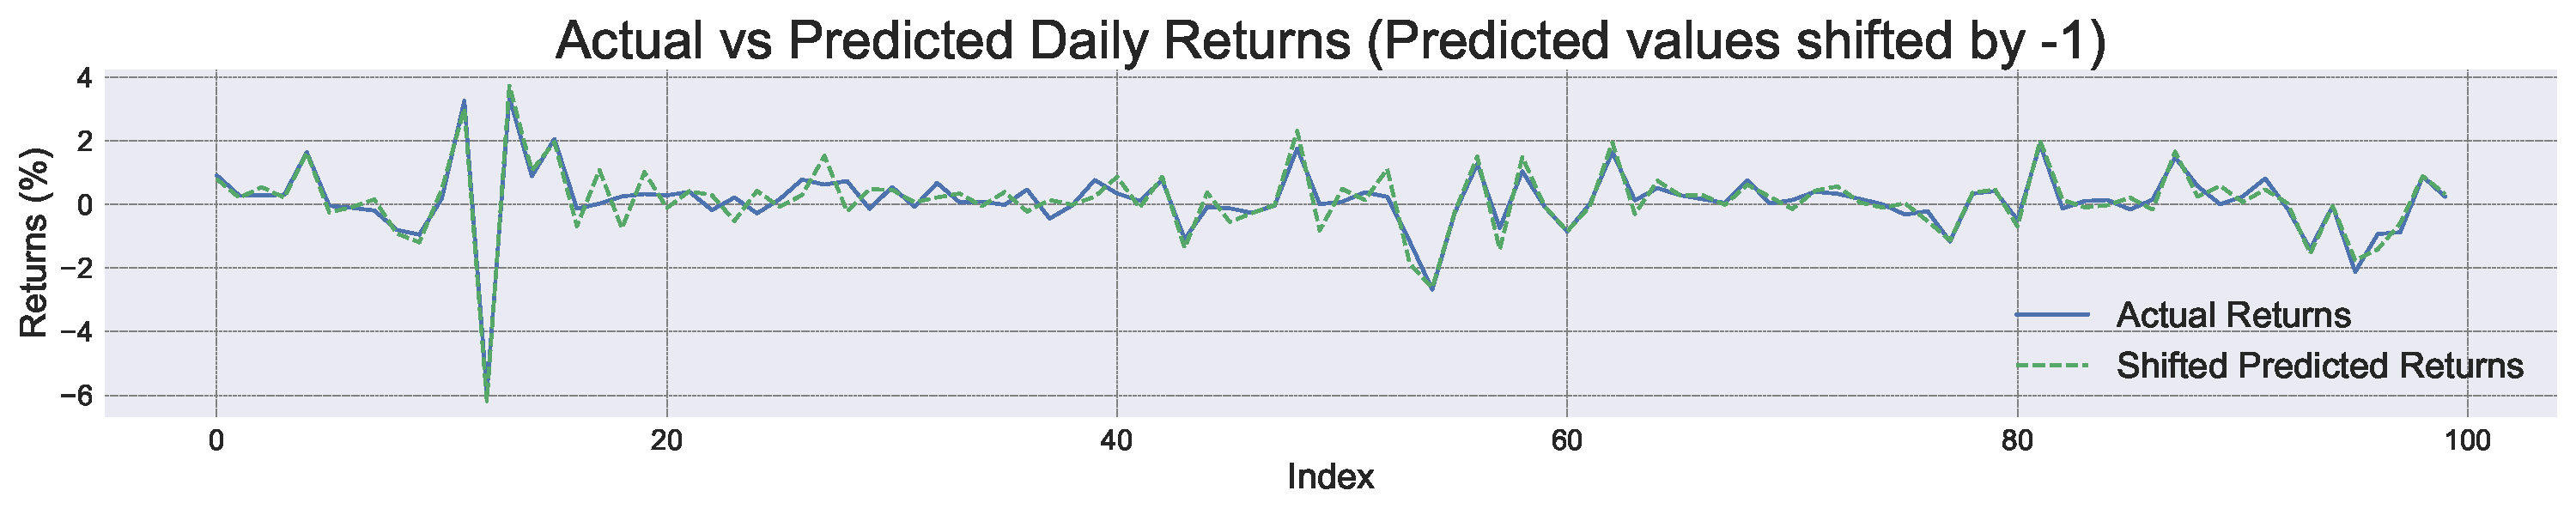
\includegraphics[width=\textwidth]{23MAI004_Sem3_MidSem_Report/returns_comparisionshift.pdf}
%     \caption{  Returns: Shifted Predictions (-1)}
%     \label{fig:revisedApproachshift2}
% \end{figure}

% Table~\ref{tab:lstm_rls_shift} shows the RMSE comparison between Hybrid LSTM-RLS predicted daily close-based calculated returns and Hybrid LSTM-RLS predicted shifted daily close-based calculated returns.

% \begin{table}[ht]
% \centering
% \begin{tabular}{|l|c|}
% \hline
% \multicolumn{2}{|c|}{\textbf{LSTM-RLS Error between Actual and Predicted Daily Returns}} \\ \hline
% \textbf{Original RMSE}       & 1.01\%   \\ \hline
% \textbf{RMSE with Shift - 1} & \textbf{0.24\%} \\ \hline
% \end{tabular}
% \caption{RMSE Comparison for Daily Returns (LSTM-RLS)}
% \label{tab:lstm_rls_shift}
% \end{table}

% \section{DNS Architecture Results}

% Figure~\ref{fig:DNSplot} shows the best actual vs predicted plot when trained and tested on the DNS architecture to remove lag in prediction.

% % Modify figure sizes according to your needs
% \begin{figure}[h!]
%     \centering
%     \includegraphics[width=\textwidth]{23MAI004_Sem3_MidSem_Report/actual_vs_predicted_main_N2_50seq_LSTM.pdf}
%     \caption{ Comparison of Stock Prices and Returns (Shifted -1)}
%     \label{fig:DNSplot}
% \end{figure}

% Table~\ref{tab:DNSres} shows the RMSE and R2 results for the DNS architecture with all combination of networks used.

% \begin{table}[ht]
% \centering
% \begin{tabular}{|l|c|c|c|c|}
% \hline
% \textbf{DNS}     & \textbf{LSTM-SDM} & \textbf{LSTM-MA} & \textbf{RBF-SDM} & \textbf{RBF-MA} \\ \hline
% \textbf{RMSE}    & 1082.0187          & 688.529          & \textbf{328.7387}         & 479.8617        \\ \hline
% \textbf{R2}      & 0.8092             & 0.9227           & \textbf{0.9823}  & 0.9624          \\ \hline
% \end{tabular}
% \caption{Comparison of DNS Models: LSTM-SDM, LSTM-MA, RBF-SDM, and RBF-MA}
% \label{tab:DNSres}
% \end{table}

% \section{Publication}
% The paper based on this work has been selected for presentation at the \textbf{28th Nirma International Conference on Management (NICOM)}. The conference will be held from \textbf{January 8 to January 10, 2024}, and the work will be presented under the sub-theme of \textbf{Finance and Accounting}. Specifically, the presentation falls under the track titled \textit{"Financial Technologies and Digitalization: Financial Analytics and Machine Learning \& Deep Learning Applications in Finance."}


\chapter{Results and Evaluation}

\section{Evaluation Metrics and Criteria}

\subsection*{Root Mean Squared Error (RMSE)}
The Root Mean Squared Error (RMSE) is a criterion used to evaluate the accuracy of the model’s forecast. It is calculated as the square root of the arithmetic mean of the squared differences between actual and predicted values. RMSE provides insights into the scale of errors, especially for regression models. It is defined as:

\begin{equation}
\text{RMSE} = \sqrt{\frac{1}{n} \sum_{i=1}^{n} (y_i - \hat{y}_i)^2}
\end{equation}

where:
\begin{itemize}
    \item \( n \): Number of observations
    \item \( y_i \): Actual value of the \(i^{th}\) observation
    \item \( \hat{y}_i \): Predicted value of the \(i^{th}\) observation
\end{itemize}

\subsection*{R-squared (R²)}
The coefficient of determination, \(R^2\), measures the proportion of variance in the dependent variable explained by the model. Its range is from 0 to 1, where 1 indicates that the model explains all the variation, and 0 indicates no explanatory power. It is defined as:

\begin{equation}
R^2 = 1 - \frac{\sum_{i=1}^{n} (y_i - \hat{y}_i)^2}{\sum_{i=1}^{n} (y_i - \bar{y})^2}
\end{equation}

where:
\begin{itemize}
    \item \( n \): Number of observations
    \item \( y_i \): True value of the \(i^{th}\) observation
    \item \( \hat{y}_i \): Predicted value of the \(i^{th}\) observation
    \item \( \bar{y} \): Mean of the actual values
\end{itemize}

\section{Performance of Enhanced Hybrid LSTM-RLS Architecture}

\subsection{Results Before and After Shift Adjustment}

\begin{figure}[h!]
    \centering
    \includegraphics[width=\textwidth]{Images/ActvsPred.pdf}
    \caption{Original vs. Predicted Stock Prices}
    \label{fig:refinedApproachRes1}
\end{figure}

\begin{figure}[h!]
    \centering
    \includegraphics[width=\textwidth]{Images/returns_comparision.pdf}
    \caption{Returns: Original vs. Predicted Prices}
    \label{fig:refinedApproachRes2}
\end{figure}

\begin{table}[h!]
\centering
\caption{LSTM-RLS Performance Metrics}
\begin{tabular}{|l|c|c|c|}
\hline
\textbf{LSTM-RLS}  & \textbf{Daily Returns} & \textbf{Weekly Returns} & \textbf{Daily Close} \\ \hline
\textbf{RMSE}      & 0.76\%                 & 1.44\%                 & 161.8935             \\ \hline
\textbf{R2}        & -0.0636                & -0.038                 & 0.9956               \\ \hline
\end{tabular}

\label{tab:lstm_rls_performance}
\end{table}

\begin{figure}[h!]
    \centering
    \includegraphics[width=\textwidth]{Images/ActvsPredshift.pdf}
    \caption{Stock Prices: Shifted Predictions (-1)}
    \label{fig:revisedApproachshift1}
\end{figure}

\begin{table}[h!]
\centering
\caption{RMSE Comparison for Daily Returns (LSTM-RLS)}
\begin{tabular}{|l|c|}
\hline
\multicolumn{2}{|c|}{\textbf{LSTM-RLS Error between Actual and Predicted Daily Returns}} \\ \hline
\textbf{Original RMSE}       & 1.01\%   \\ \hline
\textbf{RMSE with Shift - 1} & \textbf{0.24\%} \\ \hline
\end{tabular}

\label{tab:lstm_rls_shift}
\end{table}

\subsection{Performance with Multi-Feature Dataset}

\begin{figure}[h!]
    \centering
    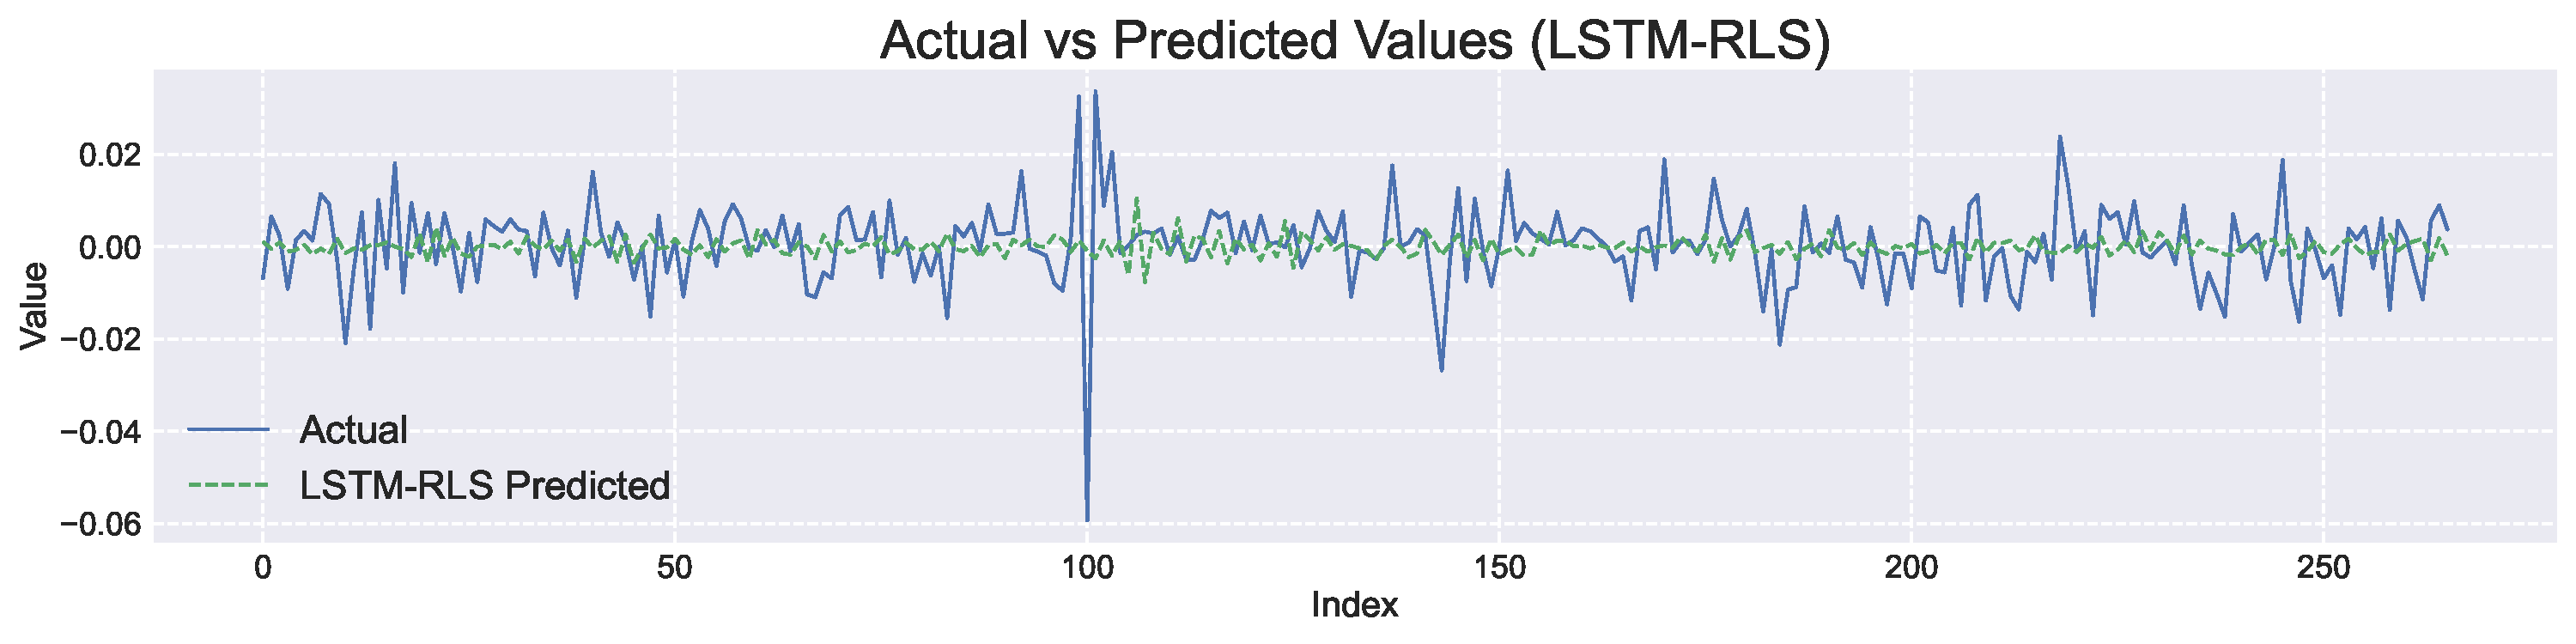
\includegraphics[width=\textwidth]{Images/5_ActvsPred_LSTM_RLS.pdf}
    \caption{Stock Prices: Actual vs. Predicted Daily Returns}
    \label{fig:actvspred_returns}
\end{figure}

\begin{table}[h!]
\centering
\caption{Performance Metrics for Multi-Feature LSTM-RLS}
\label{tab:performance_metrics}
\begin{tabular}{|l|c|}
\hline
\textbf{Metric}   & \textbf{Value}  \\ \hline
RMSE              & 0.91\%  \\ \hline
R\textsuperscript{2} Score & -0.061  \\ \hline
\end{tabular}
\end{table}

\section{Performance of DNS Architecture}

Figure~\ref{fig:DNSplot} shows the best actual vs predicted plot when trained and tested on the DNS architecture to remove lag in prediction.

% Modify figure sizes according to your needs
\begin{figure}[h!]
    \centering
    \includegraphics[width=\textwidth]{Images/actual_vs_predicted_main_N2_50seq_LSTM.pdf}
    \caption{ Comparison of Stock Prices and Returns (Shifted -1)}
    \label{fig:DNSplot}
\end{figure}

Table~\ref{tab:DNSres} shows the RMSE and R2 results for the DNS architecture with all combination of networks used.

\begin{table}[ht]
\centering
\caption{Comparison of DNS Models: LSTM-SDM, LSTM-MA, RBF-SDM, and RBF-MA}
\begin{tabular}{|l|c|c|c|c|}
\hline
\textbf{DNS}     & \textbf{LSTM-SDM} & \textbf{LSTM-MA} & \textbf{RBF-SDM} & \textbf{RBF-MA} \\ \hline
\textbf{RMSE}    & 1082.0187          & 688.529          & \textbf{328.7387}         & 479.8617        \\ \hline
\textbf{R2}      & 0.8092             & 0.9227           & \textbf{0.9823}  & 0.9624          \\ \hline
\end{tabular}

\label{tab:DNSres}
\end{table}

\section{ARIMA-LSTM Residual Framework Results}

\subsection{ARIMAX Test Predictions}
Figures~\ref{fig:arimax_close} and \ref{fig:arimax_returns} present the test predictions from the ARIMAX model when the output variable is close price and daily returns, respectively.

\begin{figure}[h!]
    \centering
    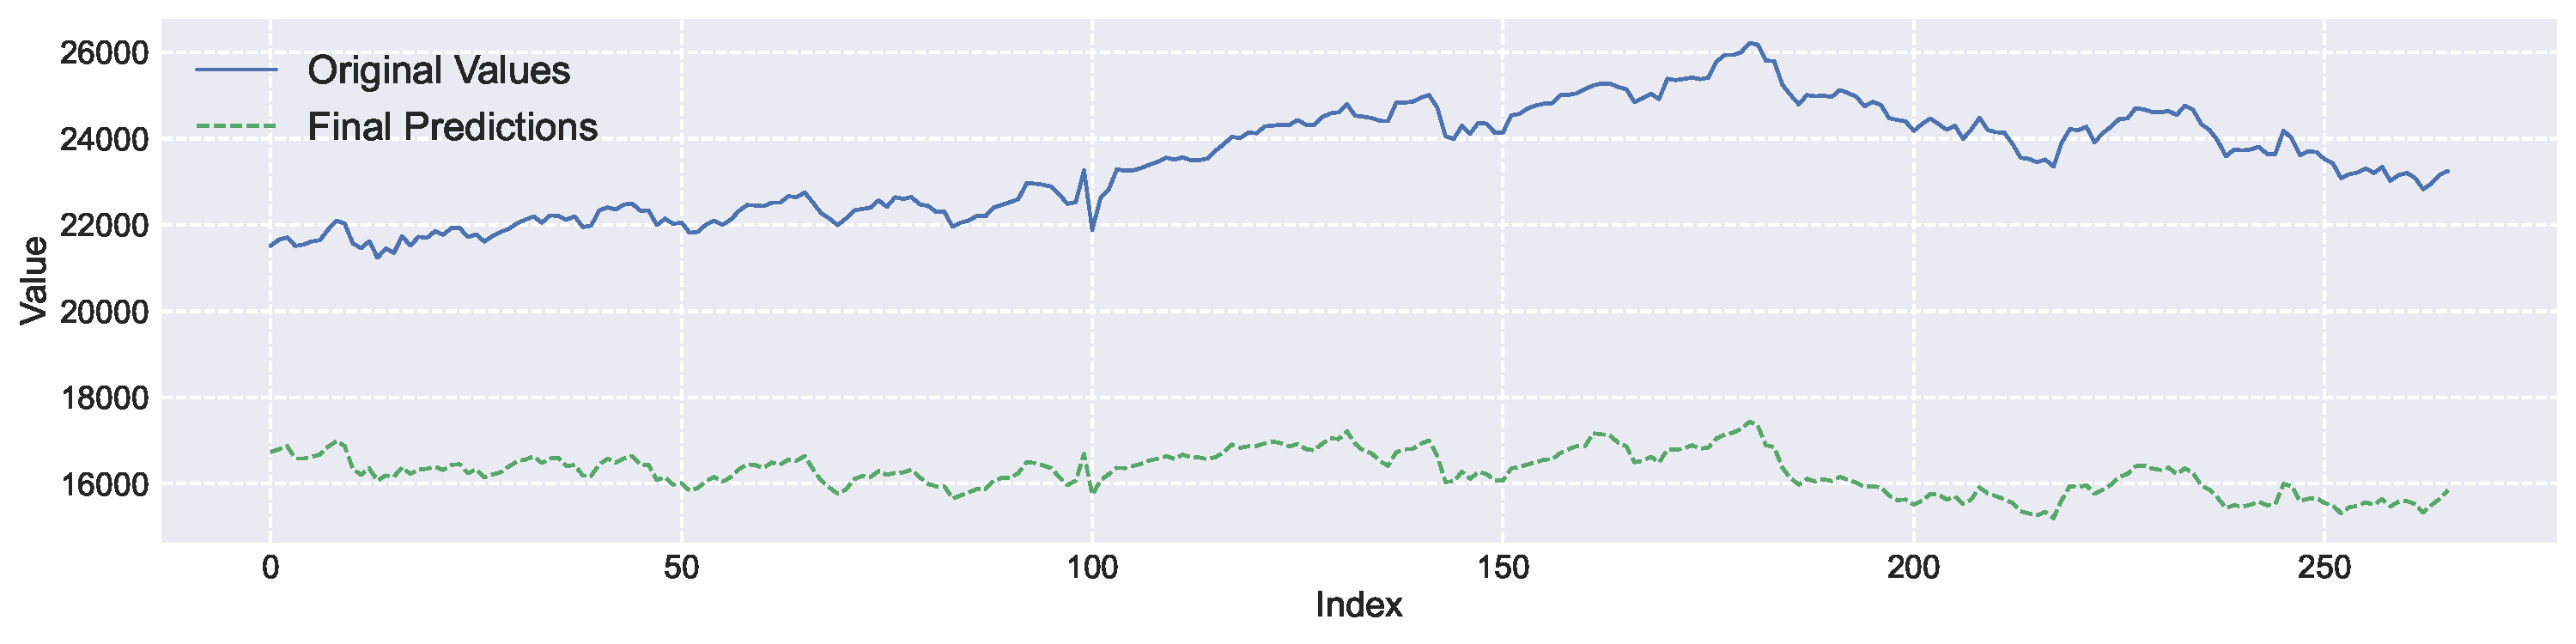
\includegraphics[width=\textwidth]{Images/3_final_predictions_close.pdf}
    \caption{ARIMAX Test Predictions - Output: Close Price}
    \label{fig:arimax_close}
\end{figure}

\begin{figure}[h!]
    \centering
    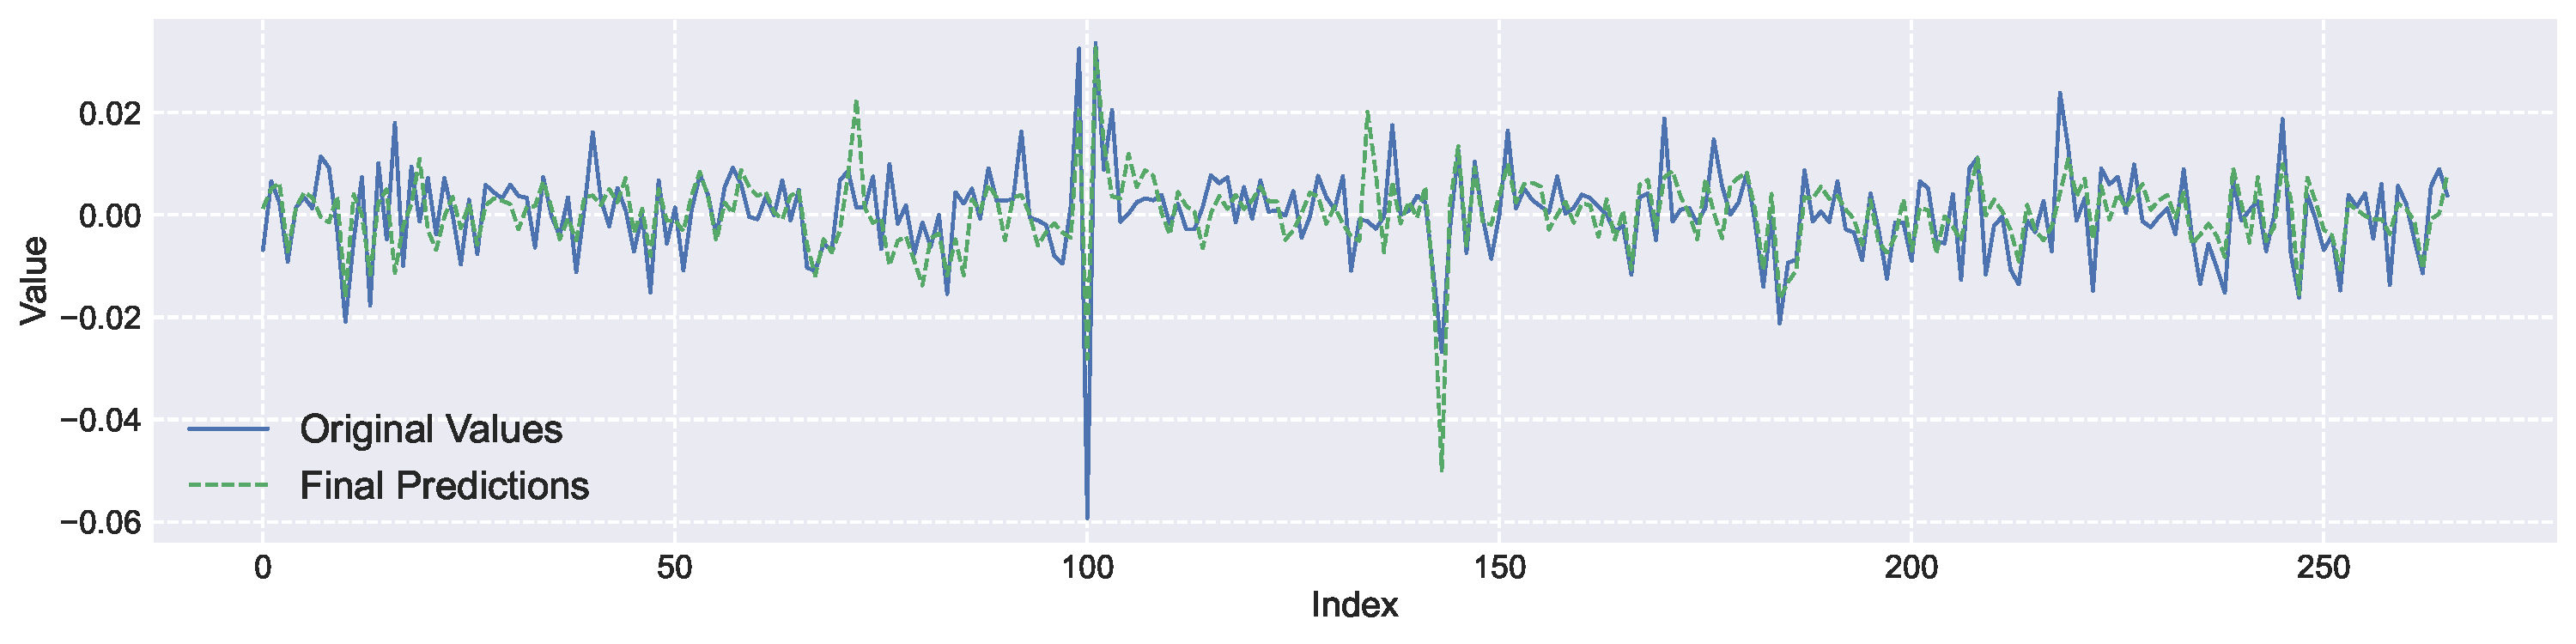
\includegraphics[width=\textwidth]{Images/3_final_predictions_return.pdf}
    \caption{ARIMAX Test Predictions - Output: Returns}
    \label{fig:arimax_returns}
\end{figure}

\subsection{Final Test Predictions}
Figures~\ref{fig:final_close} and \ref{fig:final_returns} illustrate the final test predictions after integrating LSTM when the output is close price and daily returns.

\begin{figure}[h!]
    \centering
    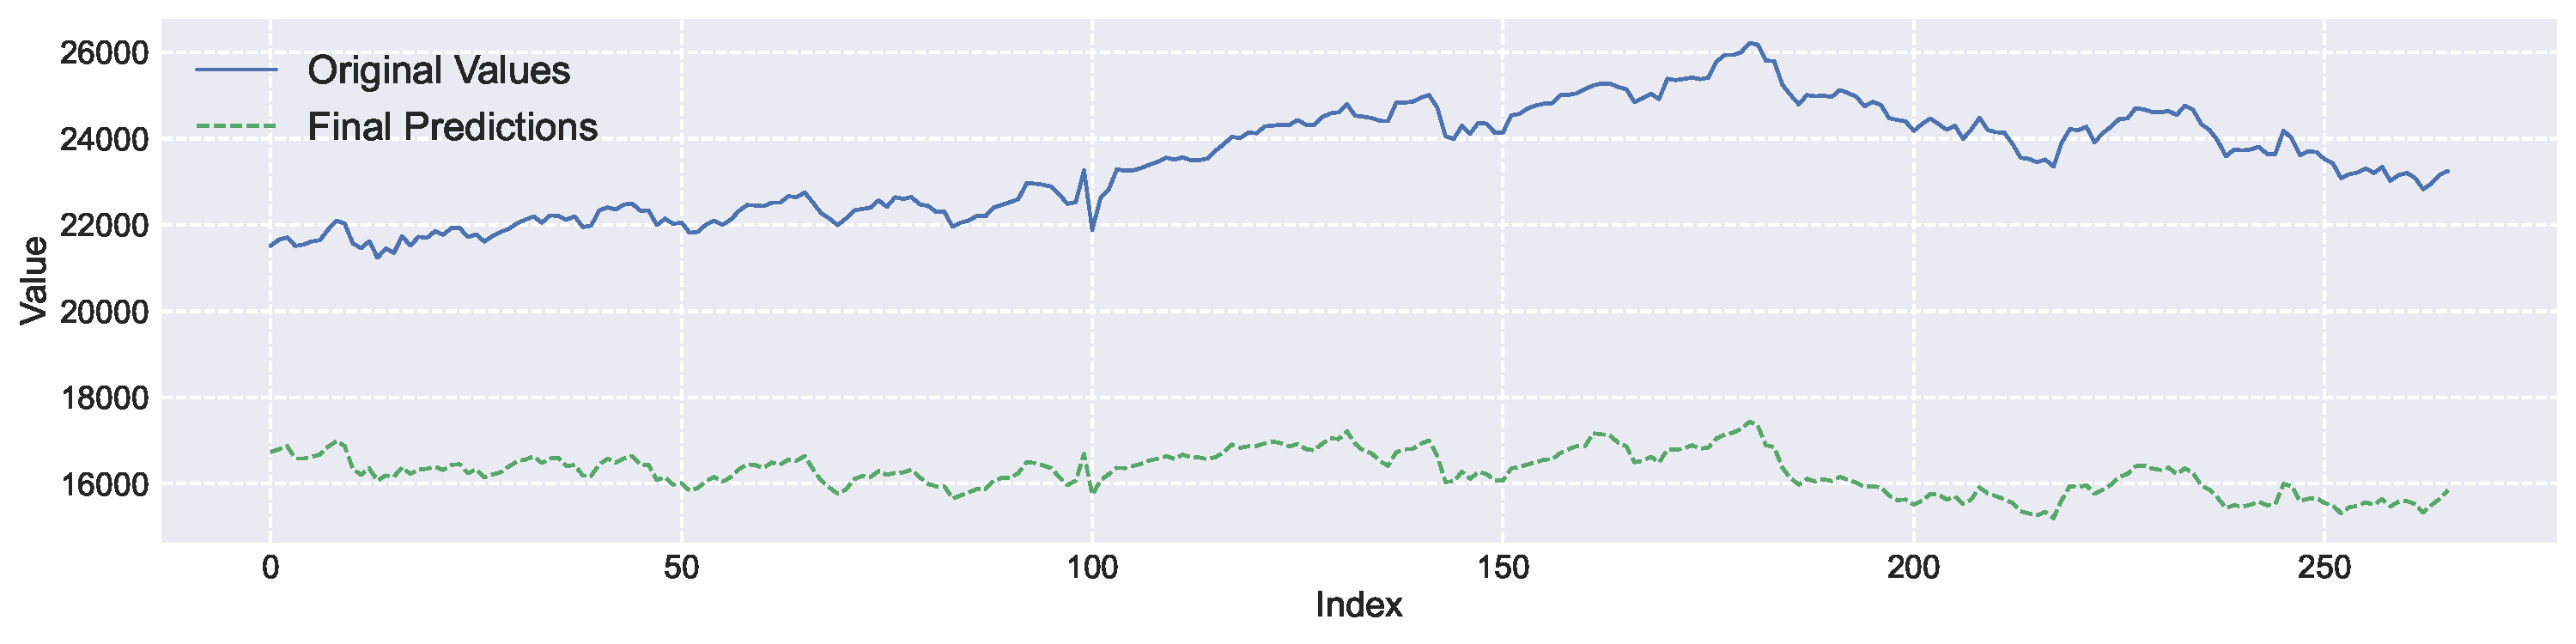
\includegraphics[width=\textwidth]{Images/3_final_predictions_close.pdf}
    \caption{Final Test Predictions - Output: Close Price}
    \label{fig:final_close}
\end{figure}

\begin{figure}[h!]
    \centering
    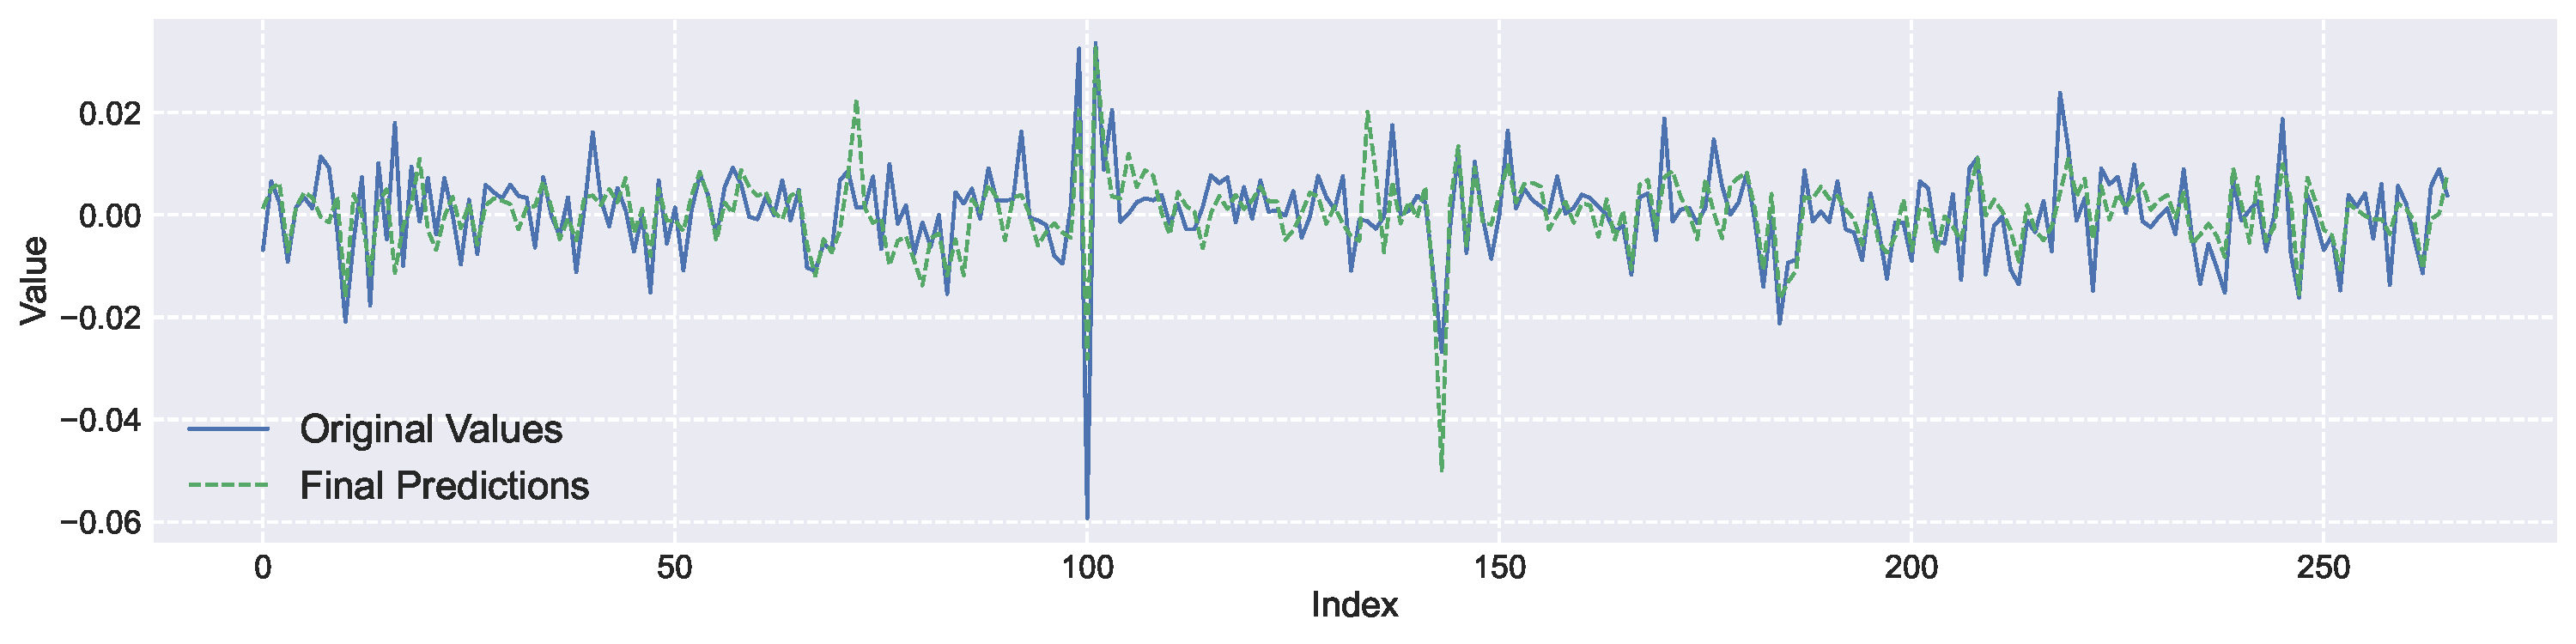
\includegraphics[width=\textwidth]{Images/3_final_predictions_return.pdf}
    \caption{Final Test Predictions - Output: Returns}
    \label{fig:final_returns}
\end{figure}

\subsection{Performance Metrics}
Table~\ref{tab:performance_arimax_final} compares the test RMSE and \( R^2 \) scores for ARIMAX and the final model when predicting close prices and daily returns.

\begin{table}[h!]
\centering
\caption{Test RMSE and \( R^2 \) Score for ARIMAX and Final Model}
\label{tab:performance_arimax_final}
\begin{tabular}{|l|c|c|}
\hline
\textbf{Model} & \textbf{RMSE} & \textbf{\( R^2 \) Score} \\ \hline
ARIMAX (Close) & 7431.43 & -35.47 \\ \hline
ARIMAX (Returns) & 0.703\% & 0.36 \\ \hline
Final Model (Close) & 7394.61 & -35.11 \\ \hline
Final Model (Returns) & 0.669\% & 0.42 \\ \hline
\end{tabular}
\end{table}

\subsection{Impact of RLS on Final Predictions}

\begin{figure}[h!]
    \centering
    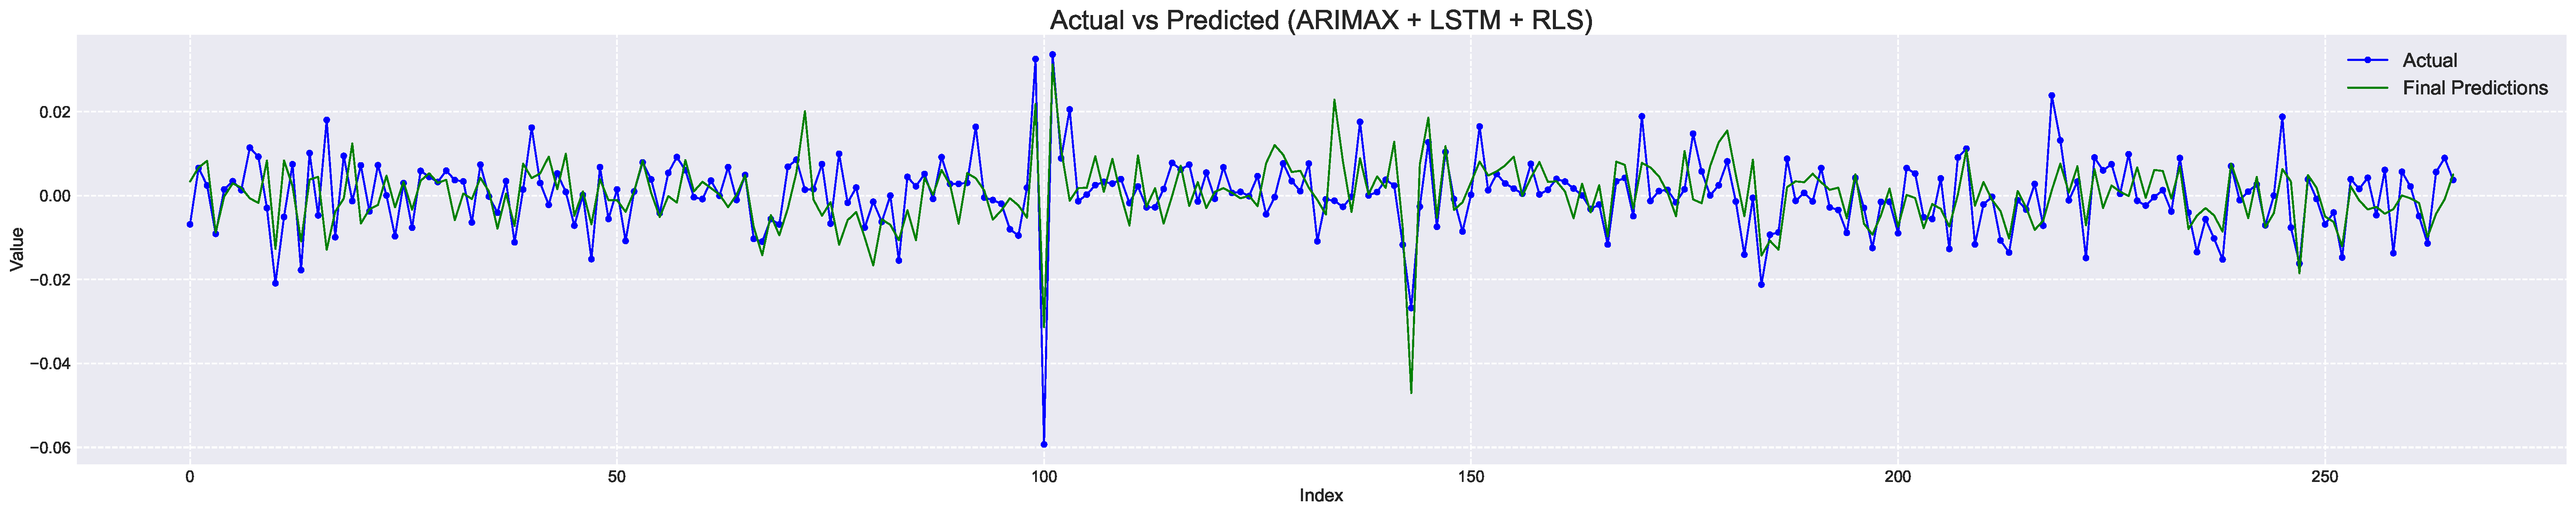
\includegraphics[width=\textwidth]{Images/6_Final_Pred.pdf}
    \caption{Actual vs. Predicted Returns After Applying RLS to Final Predictions}
    \label{fig:rls_on_residuals}
\end{figure}

\begin{table}[h!]
\centering
\caption{Performance Metrics After Applying RLS to Residuals}
\label{tab:rls_residuals_performance}
\begin{tabular}{|l|c|}
\hline
\textbf{Metric}   & \textbf{Value}  \\ \hline
RMSE              & 0.72\%  \\ \hline
R\textsuperscript{2} Score & 0.32  \\ \hline
\end{tabular}
\end{table}

\section{Multi-Feature LSTM Results}
This section presents the evaluation results of the Multi-Feature LSTM Forecasting Framework, focusing on its performance in predicting daily close returns. The evaluation metrics and visualizations demonstrate the accuracy and adaptability of the framework, as well as its ability to handle real-time updates as per the incremental training methodology discussed earlier.

\subsection{Evaluation Metrics and Analysis}
The framework's performance is evaluated using two key visualizations:
\begin{enumerate}
    \item \textbf{Absolute Error vs Total RMSE:} Figure~\ref{fig:absolute_error_rmse} plots the absolute error between actual and predicted daily close returns in one time step prediction. Besides, it plots the total RMSE of the test set for the entire duration of evaluation. This graph plots how well the architecture minimizes the errors from predictions.

    \item \textbf{Actual vs Predicted Close Returns:} Figure~\ref{fig:actual_vs_predicted} depicts the agreement
Between actual and predicted daily close returns with re-training of the model after every prediction following incremental training approach. The above plot indicates the learning ability of the model as well as real-time predictive accuracy.
\end{enumerate}

\subsection{Interpretation of Results}
\begin{itemize}
    \item The high absolute error values observed in Figure~\ref{fig:absolute_error_rmse} verify that the model is not very good at predicting daily close returns.
    \item The difference between the actual and predicted returns in  Figure~\ref{fig:actual_vs_predicted} is a result of how the incremental training works, allowing the model to capture recent market trends.
    \item A comparison of absolute error with total RMSE clearly highlights the significance of one-time step prediction error minimization for successful application in algorithmic trading.
\end{itemize}

\subsection{Visualization of Results}
The plots illustrating the framework's performance are provided below:

\begin{figure}[h!]
    \centering
    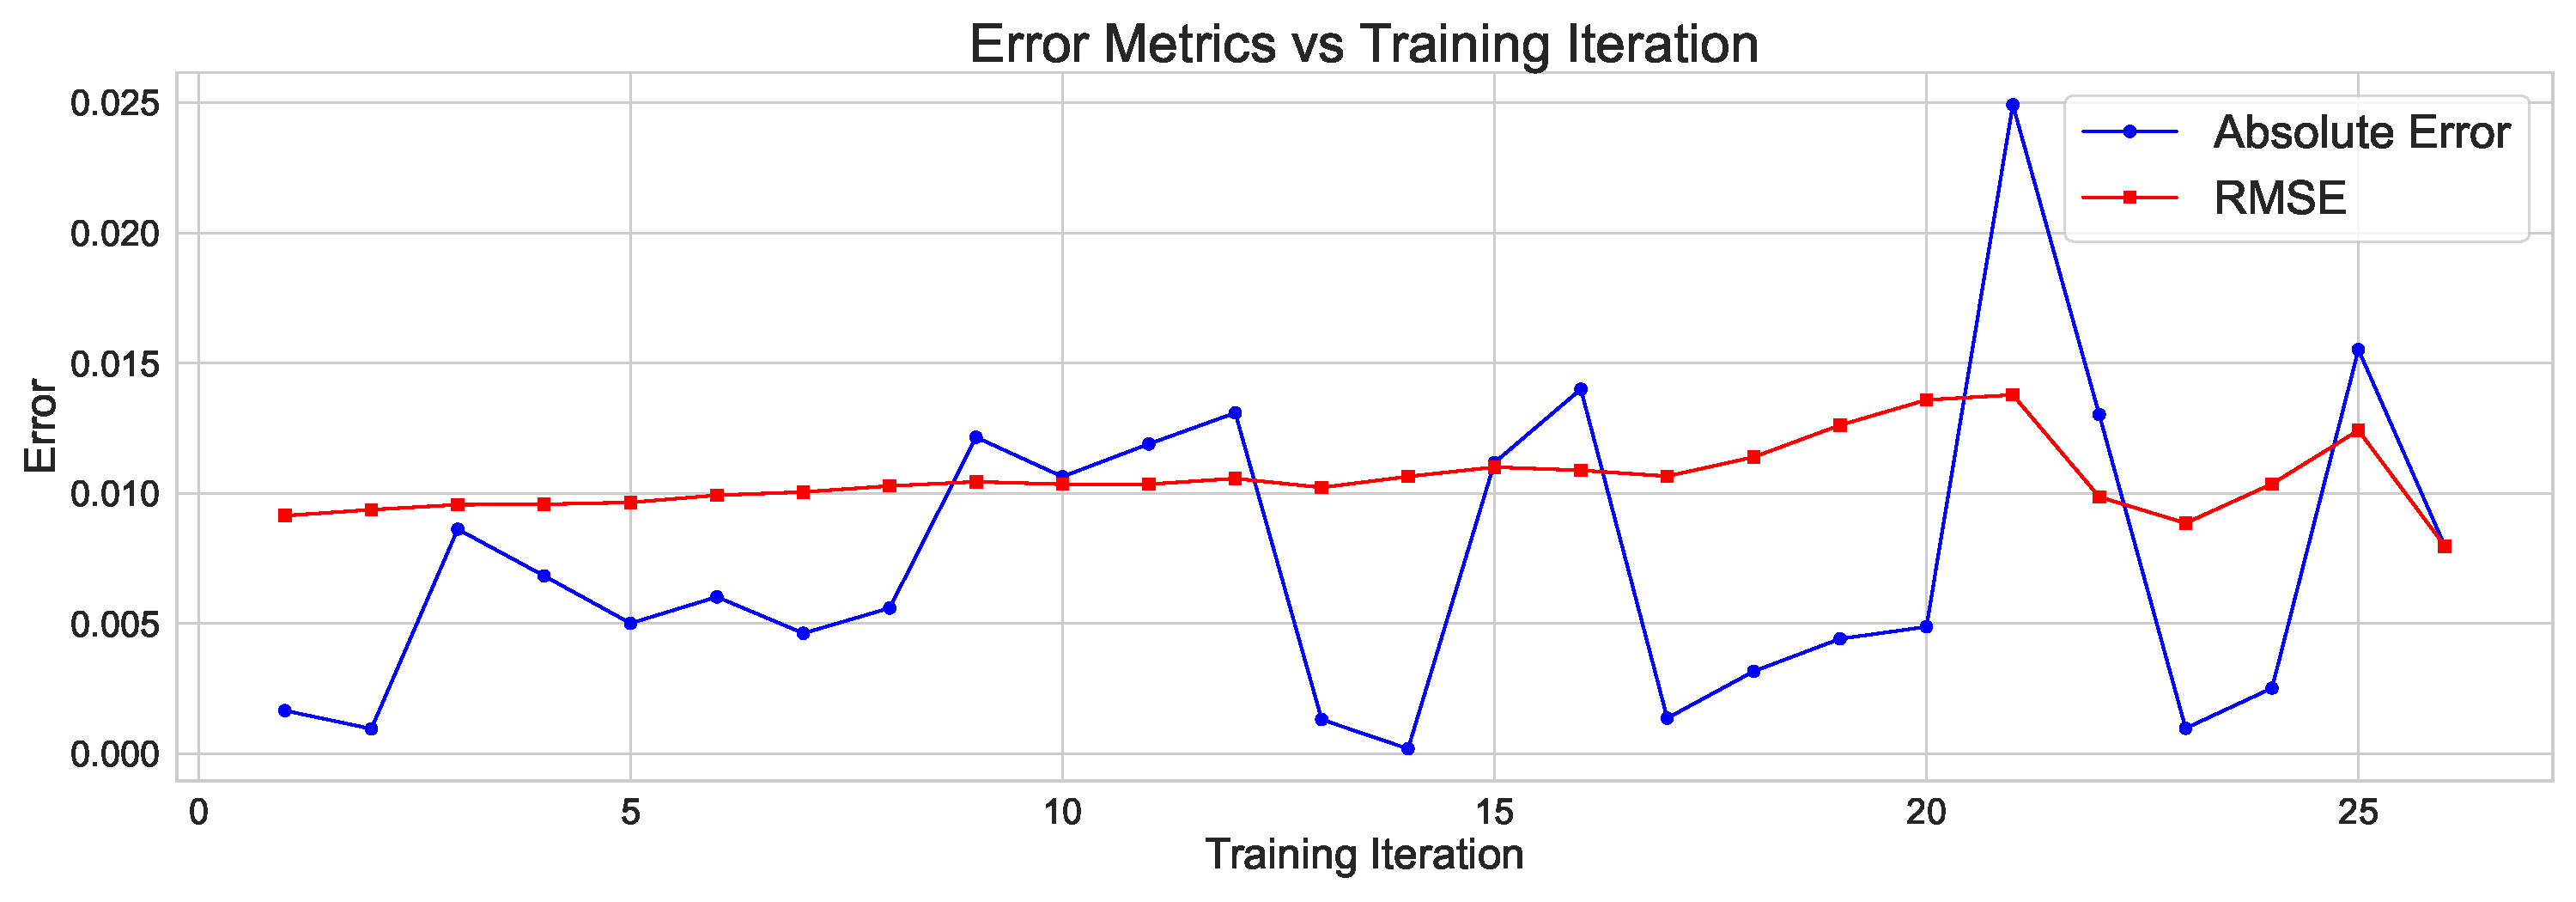
\includegraphics[width=\textwidth]{Images/absolute_error_vs_rmse.pdf}
    \caption{Absolute error between actual and predicted one-time step daily close return, compared with the total RMSE of the test data.}
    \label{fig:absolute_error_rmse}
\end{figure}

\begin{figure}[h!]
    \centering
    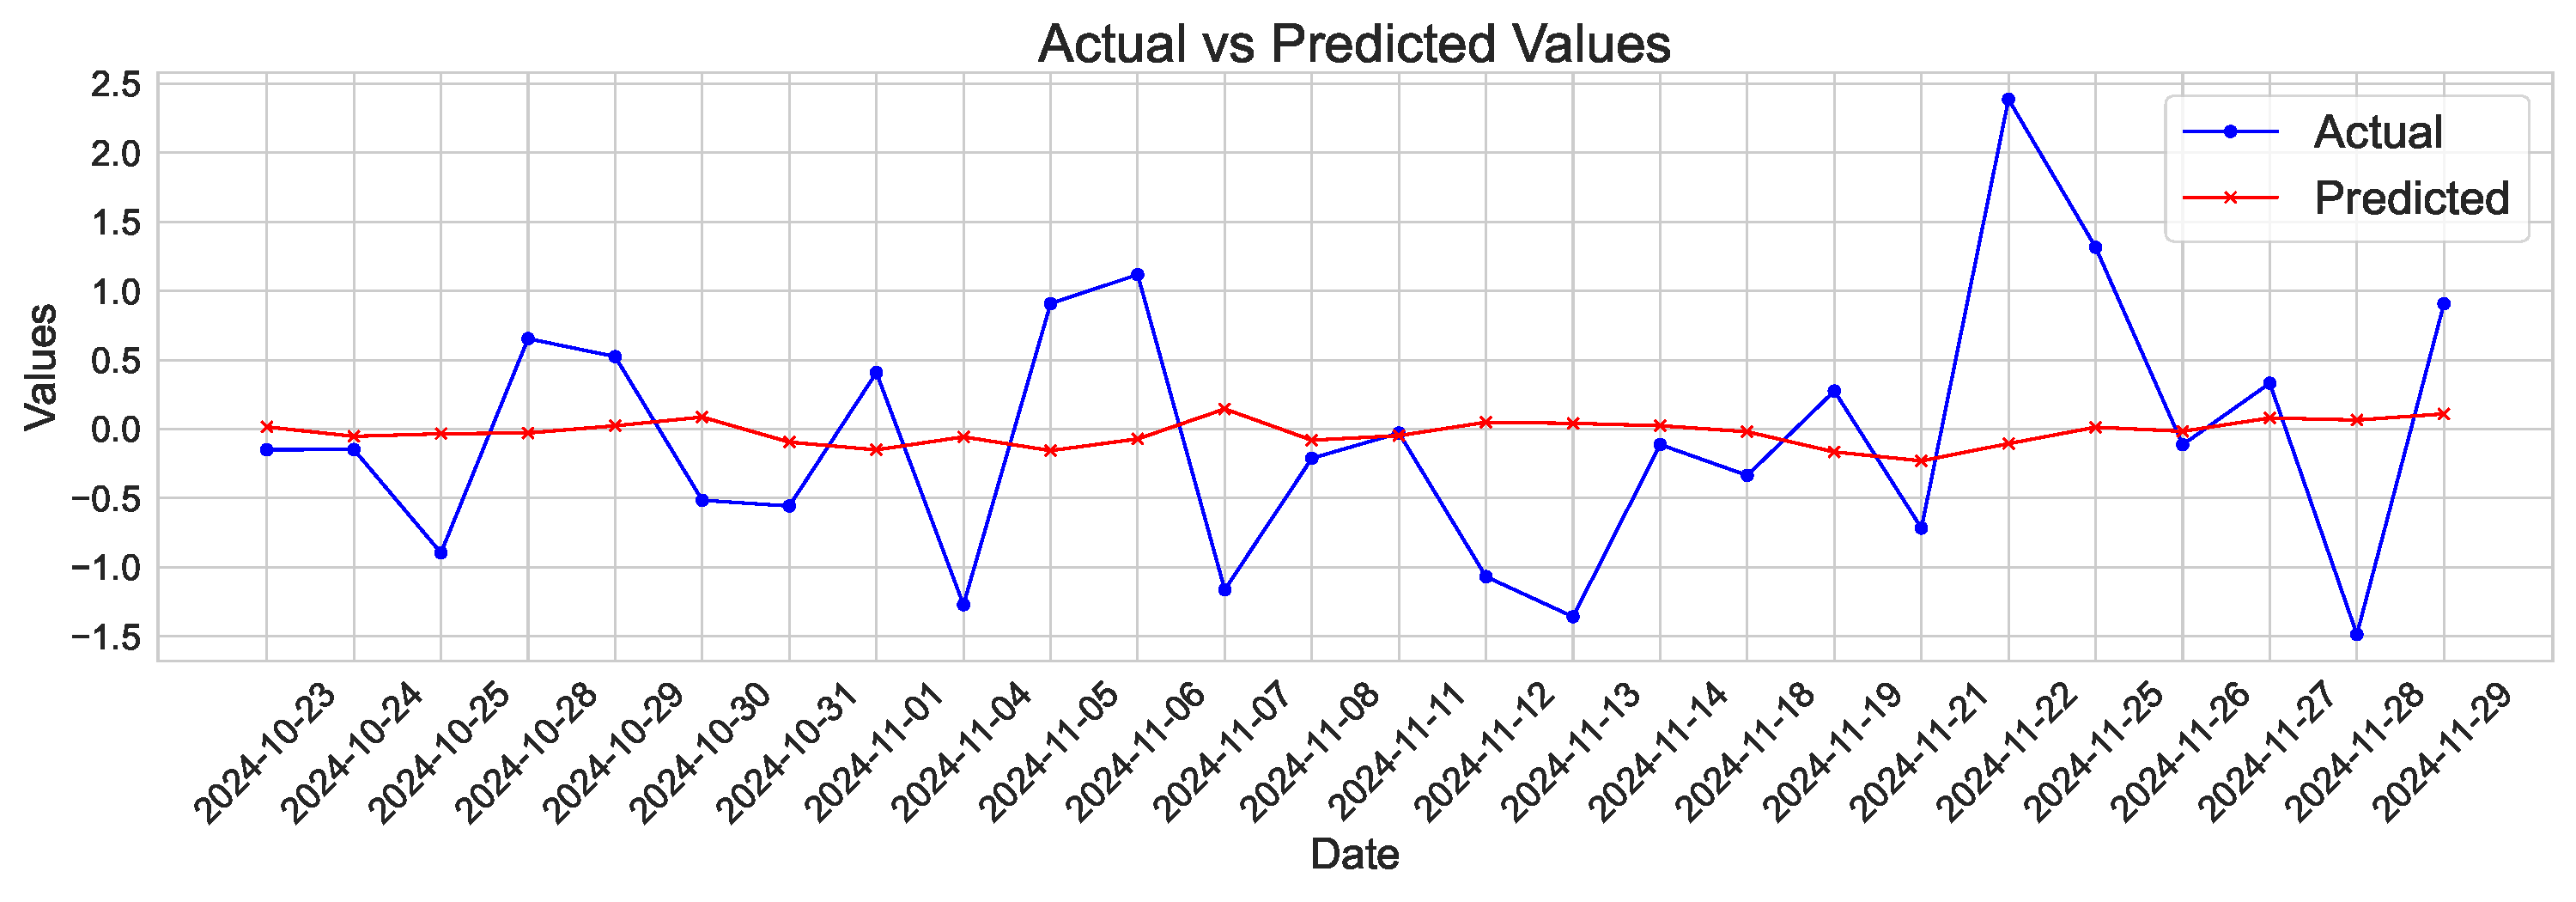
\includegraphics[width=\textwidth]{Images/actual_vs_predicted_returns.pdf}
    \caption{Actual vs Predicted daily close return where the model is retrained after each prediction as per the incremental training methodology.}
    \label{fig:actual_vs_predicted}
\end{figure}

\section{GARCH Model Results}

\subsection{Evaluation Metrics and Performance}

The GARCH model does not capture any volatility from the residuals, resulting in final predictions that are nearly identical to the ARIMAX model outputs.

\subsection{Residuals from ARIMAX Predictions}

To analyze the deviations captured by the GARCH model, we plot the residuals obtained by subtracting ARIMAX predictions from the actual values.

\begin{figure}[h!]
    \centering
    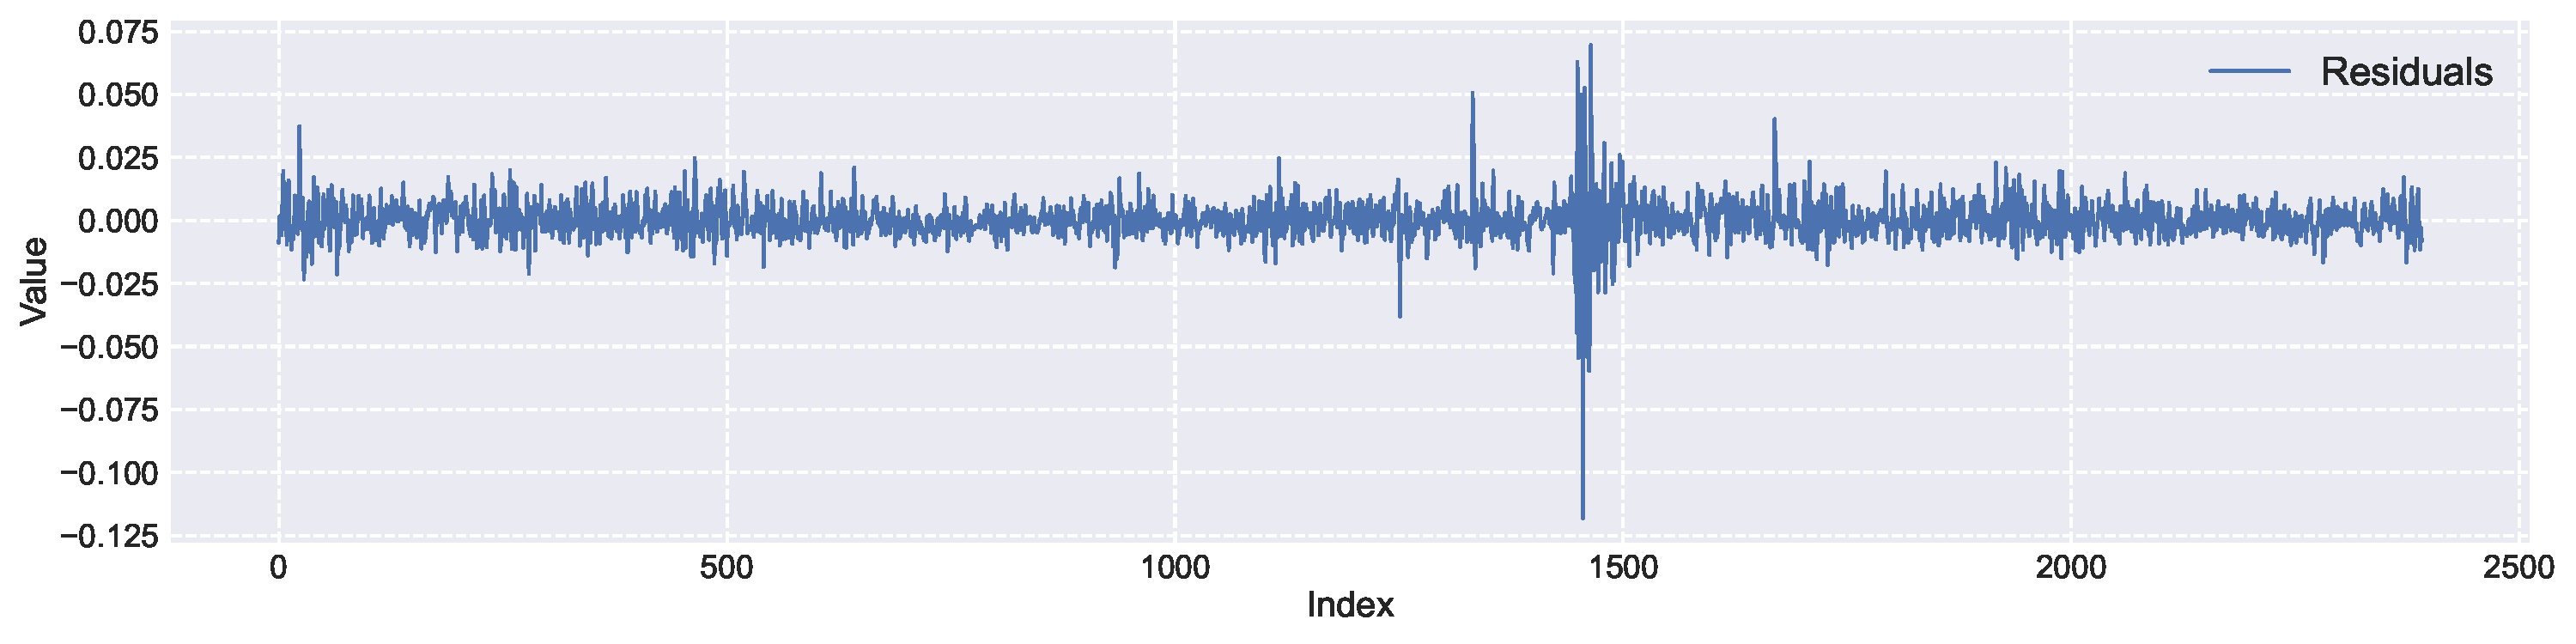
\includegraphics[width=\textwidth]{Images/7_Residuals.pdf}
    \caption{Residuals: Actual Values - ARIMAX Predictions}
    \label{fig:residuals_actual_arimax}
\end{figure}

\subsection{Visualization of Predictions}

\begin{figure}[h!]
    \centering
    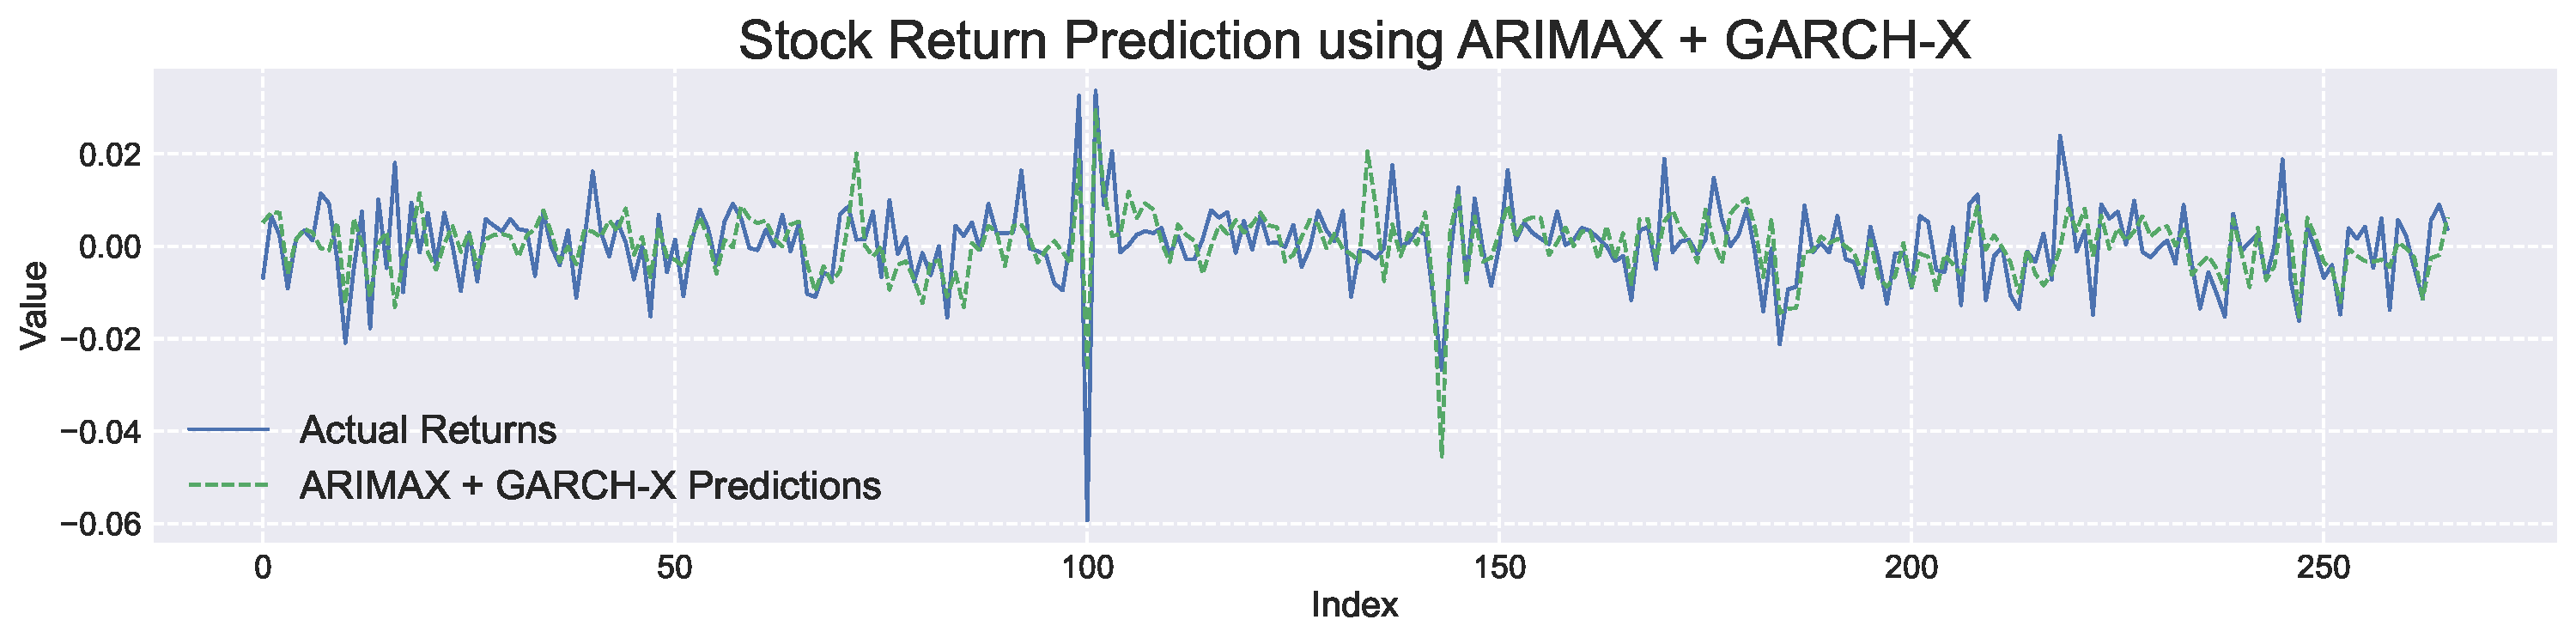
\includegraphics[width=\textwidth]{Images/7_garchx_arimax.pdf}
    \caption{Actual vs. Predicted Returns Using GARCH Model}
    \label{fig:garch_actual_pred}
\end{figure}

\begin{table}[h!]
\centering
\caption{Performance Metrics of GARCH Model}
\label{tab:garch_performance}
\begin{tabular}{|l|c|}
\hline
\textbf{Metric}   & \textbf{Value}  \\ \hline
RMSE              & 0.703\%  \\ \hline
R\textsuperscript{2} Score & 0.36  \\ \hline
\end{tabular}
\end{table}


\chapter{Discussions and Challenges}

\section{Key Findings}
Although the RMSE and \( R^2 \) score of the enhanced hybrid LSTM-RLS model were lower, the actual vs. prediction plot revealed a constant lag of one time step in the predicted stock prices. To address this issue, the DNS architecture was adopted. However, despite experimenting with various combinations of activation functions and slope trend methods, the model could not eliminate the lag.

Consequently, the DNS architecture was replaced by the ARIMA-LSTM Residual Integration Framework. Since ARIMA did not perform as expected in predicting the linear component, LSTM was utilized to predict both linear and non-linear components. However, this model also failed to remove the lag and exhibited a higher RMSE compared to other model architectures.

To further enhance performance, additional features were incorporated, and a dataset with multiple features was developed as described earlier. The Multi-Feature LSTM Forecasting Framework was then employed. Despite these enhancements, this model architecture, when combined with the proposed training method, was also unable to eliminate the lag in predictions.

Additionally, the Hybrid LSTM-RLS with a multi-feature input did not perform well. The reason behind this is that the LSTM output, which consists of daily returns, is highly volatile in nature, making it difficult for the model to generalize effectively.

The ARIMAX-LSTM-RLS model also slightly reduced performance, suggesting that the final predictions obtained from the residuals architecture do not serve as suitable inputs for the RLS model in an online prediction setting.

Furthermore, GARCH, for some reason, failed to capture any volatility (variance) in the residuals obtained after the mean predictions by ARIMAX. As a result, the final predictions produced by GARCH were identical to those obtained from ARIMAX alone, rendering GARCH ineffective in improving prediction performance.

Based on the comparative performance of different architectures tested in this dissertation, the residuals architecture has demonstrated the best predictive capability so far.

\section{Challenges and Model Refinement}
A significant challenge faced during the development of the hybrid models was the persistent lag in long-term predictions. Despite the efforts to refine the models, this lag continued to appear, particularly in the hybrid LSTM-RLS models. When attempting to mitigate the lag by introducing alternative models designed specifically for lag removal, the RMSE decreased, but the lag issue remained unchanged.

This issue highlights the difficulty in eliminating the lag while trying to improve accuracy in long-term predictions. The persistence of this lag, even after applying different techniques to remove it, remains a key challenge in the framework.

Additionally, the volatility modeling through GARCH did not yield the expected improvements. Since GARCH consistently predicted near-zero volatility for the residuals, it failed to contribute meaningful insights into stock price fluctuations. This outcome further emphasizes the complexity of modeling stock returns, where conventional volatility models may not always be applicable or beneficial.

Overall, while significant progress has been made in understanding and refining predictive models, challenges such as lag in predictions and ineffective volatility modeling remain open problems for future research.


\chapter{Conclusion and Future Direction}

\section{Conclusion}
In this work, various hybrid models and frameworks were developed and tested to predict stock prices with the goal of improving prediction accuracy and handling the challenges associated with stock price prediction. The initial hybrid LSTM-RLS model, although promising, encountered issues with a consistent lag in the predictions, especially in long-term forecasting. Efforts to address this lag by adopting alternative models, such as the DNS architecture and ARIMA-LSTM Residual Integration Framework, led to mixed results. While the lag issue persisted, and the RMSE did not significantly improve, valuable insights were gained regarding the limitations of these models in predicting stock prices effectively.

Subsequent improvements involved expanding the feature set to develop the Multi-Feature LSTM Forecasting Framework. Despite the additional features, the problem of lag in long-term predictions remained a challenge. The experiments conducted indicate that while hybrid models can provide useful predictions, managing the lag in predictions and achieving low RMSE for long-term forecasts is still a significant challenge.

\section{Future Direction}
Future work will focus on exploring alternative architectures and advanced techniques to address the issue of lag and further improve the performance of stock price prediction models. Additionally, incorporating more sophisticated feature engineering and model tuning strategies could enhance prediction accuracy and help overcome the challenges faced in this study.

\chapter{Publications}
The paper based on this work was presented at the \textbf{28th Nirma International Conference on Management (NICOM)}, held from \textbf{January 8 to January 10, 2025}. The presentation was part of the sub-theme \textbf{Finance and Accounting}, under the track titled “\textit{Financial Technologies and Digitalization: Financial Analytics and Machine Learning \& Deep Learning Applications in Finance.}”

\clearpage
\addcontentsline{toc}{chapter}{Bibliography}
\printbibliography

\end{document}